\documentclass{beamer}
\usetheme{Madrid}
\usecolortheme{default}

% Remove navigation symbols
\setbeamertemplate{navigation symbols}{}

% Customize headline: show current section name on left
\setbeamertemplate{headline}{
    \leavevmode%
    \hbox{%
        \begin{beamercolorbox}[wd=\paperwidth,ht=2.5ex,dp=1ex,left]{section in head/foot}%
            \hspace*{2ex}\usebeamerfont{section in head/foot}\insertsectionhead
        \end{beamercolorbox}}%
    \vskip0pt%
}

% Customize footline: title (2), date (1), page number (1)
\setbeamertemplate{footline}{
    \leavevmode%
    \hbox{%
        \begin{beamercolorbox}[wd=.5\paperwidth,ht=2.25ex,dp=1ex,center]{author in head/foot}%
            \usebeamerfont{author in head/foot}\insertshorttitle
        \end{beamercolorbox}%
        \begin{beamercolorbox}[wd=.25\paperwidth,ht=2.25ex,dp=1ex,center]{title in head/foot}%
            \usebeamerfont{title in head/foot}\insertshortdate
        \end{beamercolorbox}%
        \begin{beamercolorbox}[wd=.25\paperwidth,ht=2.25ex,dp=1ex,right]{date in head/foot}%
            \usebeamerfont{date in head/foot}\insertframenumber{} / \inserttotalframenumber\hspace*{2ex}
        \end{beamercolorbox}}%
    \vskip0pt%
}

\usepackage{graphicx}
\usepackage{amsmath}
\usepackage{tikz}
\usetikzlibrary{patterns,decorations.pathreplacing}
\usepackage{booktabs}

\title{Reinforcement Learning Applied to the Snake Game}
\subtitle{ECEN 446 - Reinforcement Learning}
\author{Elyas Al-Amri \and Ejmen Al-Ubejdij \and Ahmad Al-Moslemani \and Marwan Humaid \and Umair Gavankar \and Hamad AlDous}
\institute{Texas A\&M University}
\date{ECEN 446 (Fall 2025)}

\begin{document}

%-----------------------------------------------
% Slide 1: Cover Page
%-----------------------------------------------
\begin{frame}
    \titlepage
\end{frame}

% Speaker Notes:
% - Welcome the audience
% - Briefly introduce the team (each member can wave/nod)
% - "Today we'll be presenting our project on applying reinforcement learning algorithms to the classic Snake game"
% - "We'll cover the fundamentals of RL, explore different algorithms, and show you how our trained agents learned to play"
% - Transition: "Let's start with an introduction to what reinforcement learning actually is..."

\section{Theory of RL}
%-----------------------------------------------
% Slide 2: Section - Theory of RL
%-----------------------------------------------
\begin{frame}
    \begin{center}
        \vfill
        {\Huge \textbf{Theory of RL}}
        \vfill
    \end{center}
\end{frame}

%-----------------------------------------------
% Slide 3: What is Reinforcement Learning?
%-----------------------------------------------
\begin{frame}{What is Reinforcement Learning?}
    \textbf{Learning through interaction}
    \begin{itemize}
        \item Agent takes actions in an environment
        \item Receives rewards or penalties
        \item Goal: maximize cumulative reward
    \end{itemize}

    \vspace{0.5cm}
    \textbf{Key Components:}
    \begin{itemize}
        \item \textbf{Agent} -- the learner
        \item \textbf{Environment} -- the world
        \item \textbf{State} -- current situation
        \item \textbf{Action} -- what agent can do
        \item \textbf{Reward} -- feedback signal
    \end{itemize}
\end{frame}

% Speaker Notes:
% - "RL is a type of machine learning where an agent learns by interacting with an environment"
% - "Unlike supervised learning, there's no labeled data - the agent learns from trial and error"
% - Transition: "Let's visualize how this works..."

%-----------------------------------------------
% Slide 3: The RL Loop
%-----------------------------------------------
\begin{frame}{The RL Loop}
    \begin{center}
        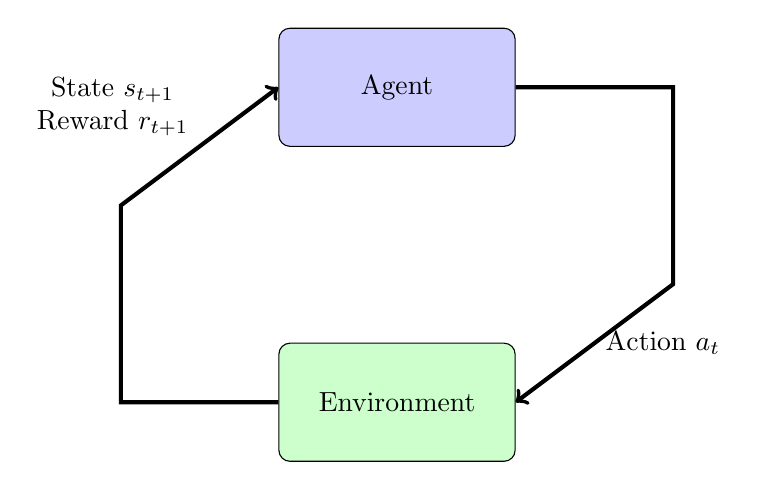
\begin{tikzpicture}[scale=1.0, every node/.style={scale=1.0}]
            % Agent
            \node[draw, rounded corners, fill=blue!20, minimum width=3cm, minimum height=1.5cm] (agent) at (0,2) {Agent};
            % Environment
            \node[draw, rounded corners, fill=green!20, minimum width=3cm, minimum height=1.5cm] (env) at (0,-2) {Environment};

            % Arrows
            \draw[->, thick, line width=1.5pt] (agent.east) -- ++(2,0) -- ++(0,-2.5) -- (env.east) node[midway, right, align=center] {Action $a_t$};
            \draw[->, thick, line width=1.5pt] (env.west) -- ++(-2,0) -- ++(0,2.5) -- (agent.west) node[midway, left, align=center, yshift=0.5cm] {State $s_{t+1}$\\Reward $r_{t+1}$};
        \end{tikzpicture}
    \end{center}

    \vspace{0.3cm}
    \begin{center}
        \textit{The agent observes, acts, and learns from feedback}
    \end{center}
\end{frame}

% Speaker Notes:
% - "This diagram shows the fundamental RL loop"
% - "The agent observes the current state, takes an action"
% - "The environment responds with a new state and a reward"
% - "Over time, it learns which actions lead to higher rewards"
% - Transition: "Now let's look at how RL has evolved over time..."

%-----------------------------------------------
% Slide 4: History of RL
%-----------------------------------------------
\begin{frame}{History of Reinforcement Learning}
    \begin{itemize}
        \item \textbf{1950s} -- Bellman: Dynamic Programming, Bellman Equation
        \item \textbf{1988} -- Sutton: Temporal Difference (TD) Learning
        \item \textbf{1989} -- Watkins: Q-Learning algorithm
        \item \textbf{1992} -- Tesauro: TD-Gammon (Backgammon)
        \item \textbf{2013} -- Mnih et al.: Deep Q-Network (DQN) plays Atari
        \item \textbf{2016} -- DeepMind: AlphaGo defeats world champion
        \item \textbf{2019} -- OpenAI Five: Beats world champions at Dota 2
        \item \textbf{2022+} -- RLHF: Training large language models
    \end{itemize}

\end{frame}

% Speaker Notes:
% - "RL has a rich history spanning over 70 years"
% - "Bellman laid the mathematical foundation with dynamic programming"
% - "The breakthrough came in 2013 when DeepMind combined deep learning with RL"
% - "DQN learned to play Atari games from raw pixels - no human knowledge needed"
% - "Today, RL is used to train large language models like ChatGPT through RLHF"
% - Transition: "Now let's see how we apply RL to our Snake game..."

%-----------------------------------------------
% Slide 5: Markov Decision Process (MDP)
%-----------------------------------------------
\begin{frame}{Markov Decision Process (MDP)}
    \textbf{Mathematical framework for RL problems}

    \vspace{0.3cm}
    An MDP is defined by a tuple $(S, A, P, R, \gamma)$:
    \begin{itemize}
        \item $S$ -- Set of \textbf{states}
        \item $A$ -- Set of \textbf{actions}
        \item $P(s'|s,a)$ -- \textbf{Transition probability}
        \item $R(s,a,s')$ -- \textbf{Reward function}
        \item $\gamma \in [0,1]$ -- \textbf{Discount factor} (importance of future rewards)
    \end{itemize}

    \vspace{0.3cm}
    \textbf{Markov Property (Memorylessness):}
    \begin{center}
        \begin{tabular}{rcl}
            MDP: & $P(s_{t+1}|s_t, a_t)$ & $= P(s_{t+1}|s_0, a_0, ..., s_t, a_t)$ \\[0.2cm]
            Exponential: & $P(X > s+t \mid X > s)$ & $= P(X > t)$
        \end{tabular}
    \end{center}

    \vspace{0.2cm}
    \textit{The future depends only on the present, not the past.}
\end{frame}

% Speaker Notes:
% - "An MDP provides the mathematical framework for RL"
% - "States describe everything the agent needs to know about the environment"
% - "Actions are what the agent can do"
% - "The transition function tells us probability of ending up in each state"
% - "The Markov property means the current state contains all relevant information"
% - Transition: "But what does this mean for Snake?"

%-----------------------------------------------
% Slide: Why Direction Matters in Snake
%-----------------------------------------------
\begin{frame}{Why Direction Matters in Snake}
    \begin{columns}
        \begin{column}{0.5\textwidth}
            \begin{center}
                \textbf{State = $(x, y)$}

                \vspace{0.3cm}
                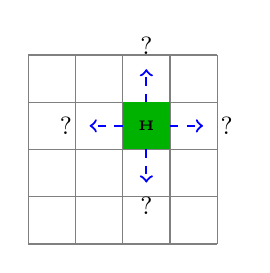
\begin{tikzpicture}[scale=0.6]
                    \draw[step=1, gray, thin] (0,0) grid (4,4);
                    \fill[green!70!black] (2,2) rectangle (3,3);
                    \node at (2.5,2.5) {\tiny \textbf{H}};
                    % Question marks for possible directions
                    \draw[->, blue, thick, dashed] (2.5,3) -- (2.5,3.7);
                    \draw[->, blue, thick, dashed] (2.5,2) -- (2.5,1.3);
                    \draw[->, blue, thick, dashed] (3,2.5) -- (3.7,2.5);
                    \draw[->, blue, thick, dashed] (2,2.5) -- (1.3,2.5);
                    \node at (2.5,4.2) {\small ?};
                    \node at (2.5,0.8) {\small ?};
                    \node at (4.2,2.5) {\small ?};
                    \node at (0.8,2.5) {\small ?};
                \end{tikzpicture}

                \vspace{0.2cm}
                {\color{red} Cannot predict next state}

                \vspace{0.1cm}
                {\small Violates Markov property}
            \end{center}
        \end{column}

        \begin{column}{0.5\textwidth}
            \begin{center}
                \textbf{State = $(x, y, v_x, v_y)$}

                \vspace{0.3cm}
                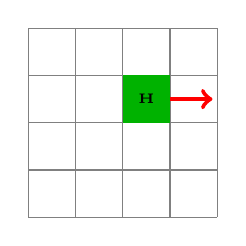
\begin{tikzpicture}[scale=0.6]
                    \draw[step=1, gray, thin] (0,0) grid (4,4);
                    \fill[green!70!black] (2,2) rectangle (3,3);
                    \node at (2.5,2.5) {\tiny \textbf{H}};
                    % Single clear direction
                    \draw[->, red, ultra thick] (3,2.5) -- (3.9,2.5);
                \end{tikzpicture}

                \vspace{0.2cm}
                {\color{green!50!black} Next state is deterministic}

                \vspace{0.1cm}
                {\small Markov property satisfied}
            \end{center}
        \end{column}
    \end{columns}

    \vspace{0.5cm}
    \begin{center}
        \textit{State must contain all information needed to predict the future.}
    \end{center}
\end{frame}

% Speaker Notes:
% - "In Snake, you can't turn 180 degrees - that's instant death"
% - "If we only store position, two identical grids could have different valid moves"
% - "By including direction, the state now tells us everything we need"
% - "This is a key insight when designing state representations"
% - Transition: "Now let's look at value functions..."

%-----------------------------------------------
% Slide: Policy Function
%-----------------------------------------------
\begin{frame}{Policy Function}
    \begin{center}
        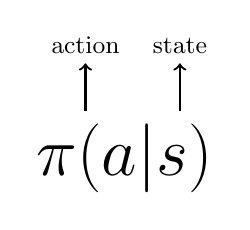
\begin{tikzpicture}
            \node at (0,0) {\Huge $\pi(a|s)$};
            % Tooltip for 'a'
            \draw[->, thick] (-0.5,0.6) -- (-0.5,1.2);
            \node[above, align=center] at (-0.5,1.2) {\small action};
            % Tooltip for 's'
            \draw[->, thick] (0.7,0.6) -- (0.7,1.2);
            \node[above, align=center] at (0.7,1.2) {\small state};
        \end{tikzpicture}
    \end{center}

    \vspace{0.5cm}
    \begin{itemize}
        \item Probability of taking action $a$ in state $s$
        \item Think of it as the agent's \textbf{strategy}
        \item \textbf{Goal:} Find optimal policy $\pi^*$ \quad {\small ($*$ denotes optimal)}
    \end{itemize}
\end{frame}

% Speaker Notes:
% - "A policy tells the agent what to do in each state"
% - "It maps states to actions (or probability distributions over actions)"
% - "Our goal in RL is to find the best policy"
% - "The asterisk notation means optimal"

%-----------------------------------------------
% Slide: Value Function
%-----------------------------------------------
\begin{frame}{Value Function}
    \begin{center}
        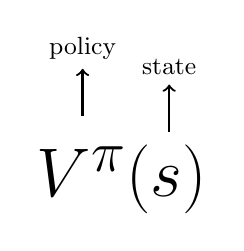
\begin{tikzpicture}
            \node at (0,0) {\Huge $V^\pi(s)$};
            % Tooltip for 'pi'
            \draw[->, thick] (-0.5,0.8) -- (-0.5,1.4);
            \node[above, align=center] at (-0.5,1.4) {\small policy};
            % Tooltip for 's'
            \draw[->, thick] (0.6,0.6) -- (0.6,1.2);
            \node[above, align=center] at (0.6,1.2) {\small state};
        \end{tikzpicture}
    \end{center}

    \vspace{0.5cm}
    \begin{itemize}
        \item Expected cumulative reward starting from state $s$
        \item Think of it as \textbf{how good} it is to be in a state
        \item Follows policy $\pi$ to estimate future rewards
    \end{itemize}

    \vspace{0.3cm}
    \[
    V^\pi(s) = \mathbb{E}_\pi \left[ \sum_{t=0}^{\infty} \gamma^t R_{t+1} \mid S_0 = s \right]
    \]
\end{frame}

%-----------------------------------------------
% Slide: Action-Value Function (Q-Function)
%-----------------------------------------------
\begin{frame}{Action-Value Function (Q-Function)}
    \begin{center}
        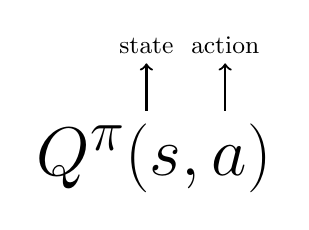
\begin{tikzpicture}
            \node at (0,0) {\Huge $Q^\pi(s, a)$};
            % Tooltip for 's'
            \draw[->, thick] (-0.1,0.6) -- (-0.1,1.2);
            \node[above, align=center] at (-0.1,1.2) {\small state};
            % Tooltip for 'a'
            \draw[->, thick] (0.9,0.6) -- (0.9,1.2);
            \node[above, align=center] at (0.9,1.2) {\small action};
        \end{tikzpicture}
    \end{center}

    \vspace{0.5cm}
    \begin{itemize}
        \item Expected cumulative reward taking action $a$ in state $s$
        \item Think of it as \textbf{how good} it is to take an action
        \item Foundation of Q-Learning and DQN
    \end{itemize}

    \vspace{0.3cm}
    \[
    Q^\pi(s,a) = \mathbb{E}_\pi \left[ \sum_{t=0}^{\infty} \gamma^t R_{t+1} \mid S_0 = s, A_0 = a \right]
    \]
\end{frame}

%-----------------------------------------------
% Slide: Bellman Equation
%-----------------------------------------------
\begin{frame}{Bellman Equation}
    \begin{center}
        {\large The recursive relationship that makes RL possible}
    \end{center}

    \vspace{0.3cm}
    \begin{center}
        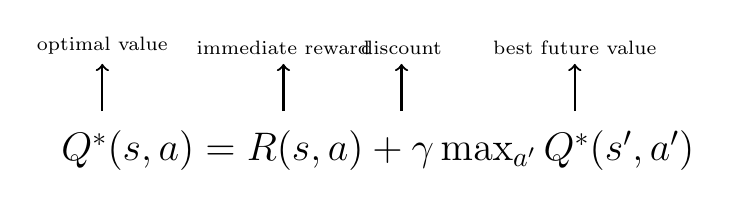
\begin{tikzpicture}
            \node at (0,0) {\Large $Q^*(s,a) = R(s,a) + \gamma \max_{a'} Q^*(s',a')$};
            % Tooltip for Q*(s,a)
            \draw[->, thick] (-3.5,0.5) -- (-3.5,1.1);
            \node[above, align=center] at (-3.5,1.1) {\scriptsize optimal value};
            % Tooltip for R(s,a)
            \draw[->, thick] (-1.2,0.5) -- (-1.2,1.1);
            \node[above, align=center] at (-1.2,1.1) {\scriptsize immediate reward};
            % Tooltip for gamma
            \draw[->, thick] (0.3,0.5) -- (0.3,1.1);
            \node[above, align=center] at (0.3,1.1) {\scriptsize discount};
            % Tooltip for max Q*(s',a')
            \draw[->, thick] (2.5,0.5) -- (2.5,1.1);
            \node[above, align=center] at (2.5,1.1) {\scriptsize best future value};
        \end{tikzpicture}
    \end{center}

    \vspace{0.5cm}
    \begin{itemize}
        \item Value of action = Immediate reward + Discounted future value
        \item $\gamma$ = discount factor (importance of future rewards)
        \item Optimal Q-value is the best possible expected return
    \end{itemize}

    \vspace{0.3cm}
    \begin{center}
        \textit{``The value now depends on the value later''}
    \end{center}
\end{frame}

%-----------------------------------------------
% Slide: Bellman Equation - Example
%-----------------------------------------------
\begin{frame}{Bellman Equation in Action}
    \begin{center}
        \textit{Which path gives more reward?}
    \end{center}

    \vspace{0.3cm}
    \begin{center}
        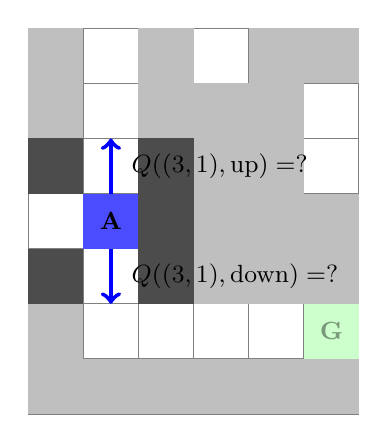
\begin{tikzpicture}[scale=0.7]
            % Grid
            \draw[step=1, gray, thin] (0,0) grid (6,7);

            % Agent is at (1,3)-(2,4), surrounding tiles: x:0-3, y:2-5
            % Adjacent walls (full opacity - within 8 surrounding tiles)
            \fill[black!70] (2,3) rectangle (3,4);  % right of agent
            \fill[black!70] (2,4) rectangle (3,5);  % top-right of agent
            \fill[black!70] (0,2) rectangle (1,3);  % bottom-left of agent
            \fill[black!70] (0,4) rectangle (1,5);  % top-left of agent

            % Foggy walls (everything else) - note: (0,3)-(1,4) is entrance, not wall
            \fill[black!25] (3,3) rectangle (6,4);  % rest of horizontal wall
            \fill[black!25] (0,0) rectangle (1,2);  % bottom of left wall
            \fill[black!25] (0,5) rectangle (1,7);  % top of left wall
            \fill[black!25] (4,6) rectangle (6,7);
            \fill[black!25] (4,4) rectangle (5,6);
            \fill[black!25] (2,5) rectangle (3,7);  % extended wall blocking upper path
            \fill[black!25] (3,4) rectangle (4,6);  % extended inner wall

            % Fill blocks around the path
            \fill[black!25] (1,0) rectangle (6,1);  % row below path (foggy)
            \fill[black!70] (2,2) rectangle (3,3);  % adjacent to agent
            \fill[black!25] (3,2) rectangle (6,3);  % row above path (foggy)

            % Goal (foggy)
            \fill[green!20] (5,1) rectangle (6,2);
            \node[opacity=0.4] at (5.5,1.5) {\small \textbf{G}};

            % Agent position (second column, 4th row)
            \fill[blue!70] (1,3) rectangle (2,4);
            \node at (1.5,3.5) {\small \textbf{A}};

            % Arrow going up from agent
            \draw[->, blue, ultra thick] (1.5,4) -- (1.5,5);
            \node[right] at (1.7,4.5) {\small $Q((3,1), \text{up}) = ?$};

            % Arrow going down from agent
            \draw[->, blue, ultra thick] (1.5,3) -- (1.5,2);
            \node[right] at (1.7,2.5) {\small $Q((3,1), \text{down}) = ?$};
        \end{tikzpicture}
    \end{center}
\end{frame}

%-----------------------------------------------
% Slide: Path Up - Step 1
%-----------------------------------------------
\begin{frame}{Bellman Equation: Path Up (Step 1)}
    \begin{center}
        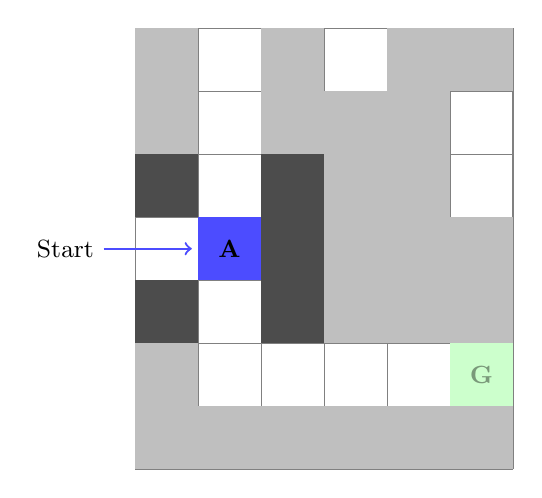
\begin{tikzpicture}[scale=0.8]
            \draw[step=1, gray, thin] (0,0) grid (6,7);

            % Walls - 8 surrounding tiles of agent are full opacity, rest are foggy
            % Agent is at (1,3)-(2,4), so surrounding tiles are x:0-3, y:2-5

            % Adjacent walls (full opacity - within 8 surrounding tiles)
            \fill[black!70] (2,3) rectangle (3,4);  % right of agent
            \fill[black!70] (2,4) rectangle (3,5);  % top-right of agent
            \fill[black!70] (0,2) rectangle (1,3);  % bottom-left of agent
            \fill[black!70] (0,4) rectangle (1,5);  % top-left of agent

            % Foggy walls (everything else)
            \fill[black!25] (3,3) rectangle (6,4);  % rest of horizontal wall
            \fill[black!25] (0,0) rectangle (1,2);  % bottom of left wall
            \fill[black!25] (0,5) rectangle (1,7);  % top of left wall
            \fill[black!25] (4,6) rectangle (6,7);
            \fill[black!25] (4,4) rectangle (5,6);
            \fill[black!25] (2,5) rectangle (3,7);  % extended wall blocking upper path
            \fill[black!25] (3,4) rectangle (4,6);  % extended inner wall

            % Fill blocks around the path
            \fill[black!25] (1,0) rectangle (6,1);  % row below path (foggy)
            \fill[black!70] (2,2) rectangle (3,3);  % adjacent to agent
            \fill[black!25] (3,2) rectangle (6,3);  % row above path (foggy)

            % Goal (foggy)
            \fill[green!20] (5,1) rectangle (6,2);
            \node[opacity=0.4] at (5.5,1.5) {\small \textbf{G}};

            % Agent (full opacity)
            \fill[blue!70] (1,3) rectangle (2,4);
            \node at (1.5,3.5) {\small \textbf{A}};

            % Start arrow
            \draw[->, thick, blue!70] (-0.5,3.5) -- (0.9,3.5);
            \node[left] at (-0.5,3.5) {\small Start};
        \end{tikzpicture}
    \end{center}
    \vspace{0.2cm}
    \begin{center}
        $Q((1,3), \text{up}) = ?$
    \end{center}
\end{frame}

%-----------------------------------------------
% Slide: Path Up - Step 2
%-----------------------------------------------
\begin{frame}{Bellman Equation: Path Up (Step 2)}
    \begin{center}
        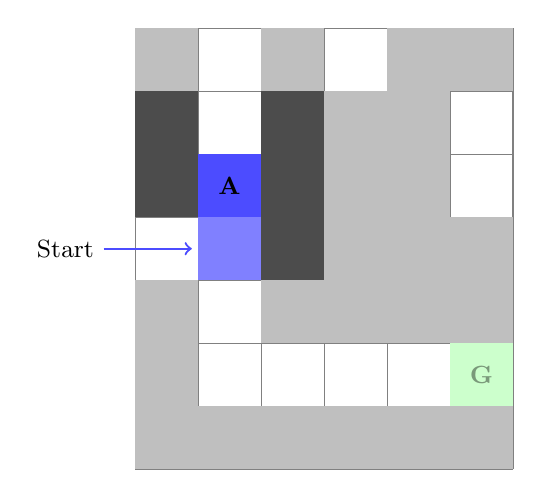
\begin{tikzpicture}[scale=0.8]
            \draw[step=1, gray, thin] (0,0) grid (6,7);

            % Agent at (1,4)-(2,5), surrounding tiles: x:0-3, y:3-6
            % Adjacent walls (full opacity) - note: (0,3)-(1,4) is entrance, not wall
            \fill[black!70] (2,3) rectangle (3,4);
            \fill[black!70] (2,4) rectangle (3,5);
            \fill[black!70] (2,5) rectangle (3,6);
            \fill[black!70] (0,4) rectangle (1,5);
            \fill[black!70] (0,5) rectangle (1,6);

            % Foggy walls
            \fill[black!25] (3,3) rectangle (6,4);
            \fill[black!25] (0,0) rectangle (1,3);
            \fill[black!25] (0,6) rectangle (1,7);
            \fill[black!25] (4,6) rectangle (6,7);
            \fill[black!25] (4,4) rectangle (5,6);
            \fill[black!25] (3,4) rectangle (4,6);  % extended inner wall
            \fill[black!25] (2,6) rectangle (3,7);  % extended wall blocking upper path

            % Fill blocks around the path (all foggy - not adjacent)
            \fill[black!25] (1,0) rectangle (6,1);  % row below path
            \fill[black!25] (2,2) rectangle (6,3);  % row above path

            % Goal (foggy)
            \fill[green!20] (5,1) rectangle (6,2);
            \node[opacity=0.4] at (5.5,1.5) {\small \textbf{G}};

            \fill[blue!50] (1,3) rectangle (2,4);
            \fill[blue!70] (1,4) rectangle (2,5);
            \node at (1.5,4.5) {\small \textbf{A}};
            % Start arrow
            \draw[->, thick, blue!70] (-0.5,3.5) -- (0.9,3.5);
            \node[left] at (-0.5,3.5) {\small Start};
        \end{tikzpicture}
    \end{center}
    \vspace{0.2cm}
    \begin{center}
        $Q((1,4), \text{up}) = ?$
    \end{center}
\end{frame}

%-----------------------------------------------
% Slide: Path Up - Step 3
%-----------------------------------------------
\begin{frame}{Bellman Equation: Path Up (Step 3)}
    \begin{center}
        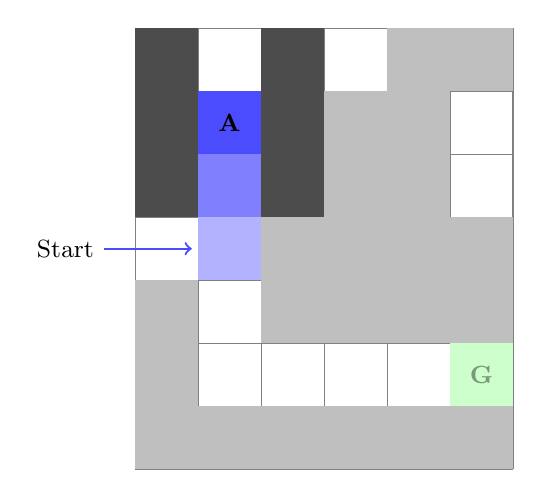
\begin{tikzpicture}[scale=0.8]
            \draw[step=1, gray, thin] (0,0) grid (6,7);

            % Agent at (1,5)-(2,6), surrounding tiles: x:0-3, y:4-7
            % Adjacent walls (full opacity)
            \fill[black!70] (2,4) rectangle (3,5);
            \fill[black!70] (2,5) rectangle (3,6);
            \fill[black!70] (2,6) rectangle (3,7);  % new wall blocking right
            \fill[black!70] (0,4) rectangle (1,5);
            \fill[black!70] (0,5) rectangle (1,6);
            \fill[black!70] (0,6) rectangle (1,7);

            % Foggy walls - note: (0,3)-(1,4) is entrance, not wall
            \fill[black!25] (2,3) rectangle (6,4);
            \fill[black!25] (0,0) rectangle (1,3);
            \fill[black!25] (4,6) rectangle (6,7);
            \fill[black!25] (4,4) rectangle (5,6);
            \fill[black!25] (3,4) rectangle (4,6);  % extended inner wall

            % Fill blocks around the path (all foggy - not adjacent)
            \fill[black!25] (1,0) rectangle (6,1);  % row below path
            \fill[black!25] (2,2) rectangle (6,3);  % row above path

            % Goal (foggy)
            \fill[green!20] (5,1) rectangle (6,2);
            \node[opacity=0.4] at (5.5,1.5) {\small \textbf{G}};

            \fill[blue!30] (1,3) rectangle (2,4);
            \fill[blue!50] (1,4) rectangle (2,5);
            \fill[blue!70] (1,5) rectangle (2,6);
            \node at (1.5,5.5) {\small \textbf{A}};
            % Start arrow
            \draw[->, thick, blue!70] (-0.5,3.5) -- (0.9,3.5);
            \node[left] at (-0.5,3.5) {\small Start};
        \end{tikzpicture}
    \end{center}
    \vspace{0.2cm}
    \begin{center}
        $Q((1,5), \text{up}) = ?$
    \end{center}
\end{frame}

%-----------------------------------------------
% Slide: Path Up - Step 4
%-----------------------------------------------
\begin{frame}{Bellman Equation: Path Up (Step 4)}
    \begin{center}
        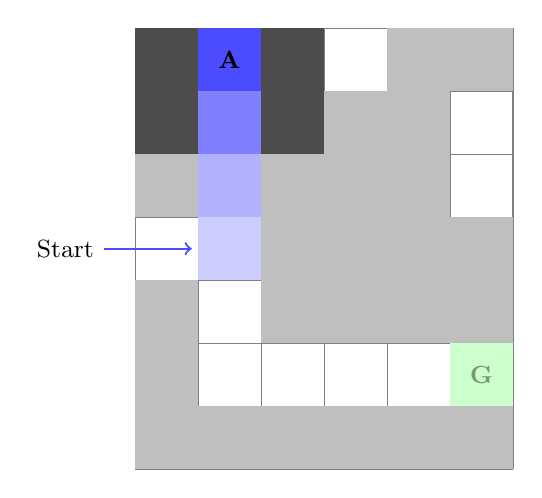
\begin{tikzpicture}[scale=0.8]
            \draw[step=1, gray, thin] (0,0) grid (6,7);

            % Agent at (1,6)-(2,7), surrounding tiles: x:0-3, y:5-7
            % Adjacent walls (full opacity)
            \fill[black!70] (2,5) rectangle (3,6);
            \fill[black!70] (2,6) rectangle (3,7);  % wall blocking right
            \fill[black!70] (0,5) rectangle (1,6);
            \fill[black!70] (0,6) rectangle (1,7);

            % Foggy walls - note: (0,3)-(1,4) is entrance, not wall
            \fill[black!25] (2,3) rectangle (6,4);
            \fill[black!25] (0,0) rectangle (1,3);
            \fill[black!25] (0,4) rectangle (1,5);
            \fill[black!25] (4,6) rectangle (6,7);
            \fill[black!25] (2,4) rectangle (3,5);
            \fill[black!25] (4,4) rectangle (5,6);
            \fill[black!25] (3,4) rectangle (4,6);  % extended inner wall

            % Fill blocks around the path (all foggy - not adjacent)
            \fill[black!25] (1,0) rectangle (6,1);  % row below path
            \fill[black!25] (2,2) rectangle (6,3);  % row above path

            % Goal (foggy)
            \fill[green!20] (5,1) rectangle (6,2);
            \node[opacity=0.4] at (5.5,1.5) {\small \textbf{G}};

            \fill[blue!20] (1,3) rectangle (2,4);
            \fill[blue!30] (1,4) rectangle (2,5);
            \fill[blue!50] (1,5) rectangle (2,6);
            \fill[blue!70] (1,6) rectangle (2,7);
            \node at (1.5,6.5) {\small \textbf{A}};
            % Start arrow
            \draw[->, thick, blue!70] (-0.5,3.5) -- (0.9,3.5);
            \node[left] at (-0.5,3.5) {\small Start};
        \end{tikzpicture}
    \end{center}
    \vspace{0.2cm}
    \begin{center}
        $Q((1,6), \text{?}) = ?$
    \end{center}
\end{frame}

%-----------------------------------------------
% Slide: Path Up - Dead End
%-----------------------------------------------
\begin{frame}{Bellman Equation: Path Up (Dead End)}
    \begin{center}
        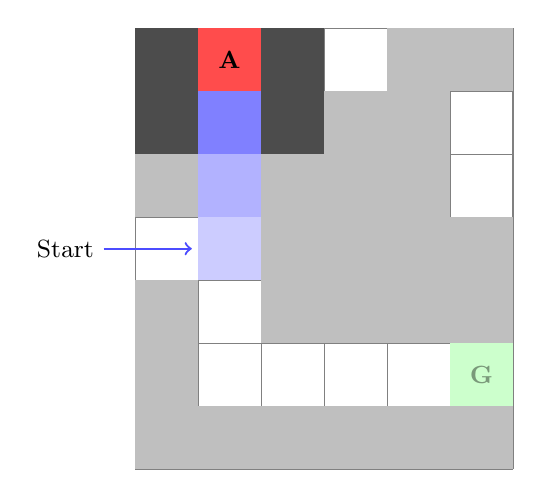
\begin{tikzpicture}[scale=0.8]
            \draw[step=1, gray, thin] (0,0) grid (6,7);

            % Agent at (1,6)-(2,7), surrounded by walls - trapped!
            % Adjacent walls (full opacity)
            \fill[black!70] (2,5) rectangle (3,6);
            \fill[black!70] (2,6) rectangle (3,7);  % wall blocking right
            \fill[black!70] (0,5) rectangle (1,6);
            \fill[black!70] (0,6) rectangle (1,7);

            % Foggy walls - note: (0,3)-(1,4) is entrance, not wall
            \fill[black!25] (2,3) rectangle (6,4);
            \fill[black!25] (0,0) rectangle (1,3);
            \fill[black!25] (0,4) rectangle (1,5);
            \fill[black!25] (4,6) rectangle (6,7);
            \fill[black!25] (2,4) rectangle (3,5);
            \fill[black!25] (4,4) rectangle (5,6);
            \fill[black!25] (3,4) rectangle (4,6);  % extended inner wall

            % Fill blocks around the path (all foggy - not adjacent)
            \fill[black!25] (1,0) rectangle (6,1);  % row below path
            \fill[black!25] (2,2) rectangle (6,3);  % row above path

            % Goal (foggy)
            \fill[green!20] (5,1) rectangle (6,2);
            \node[opacity=0.4] at (5.5,1.5) {\small \textbf{G}};

            \fill[blue!20] (1,3) rectangle (2,4);
            \fill[blue!30] (1,4) rectangle (2,5);
            \fill[blue!50] (1,5) rectangle (2,6);
            \fill[red!70] (1,6) rectangle (2,7);
            \node at (1.5,6.5) {\small \textbf{A}};
            % Start arrow
            \draw[->, thick, blue!70] (-0.5,3.5) -- (0.9,3.5);
            \node[left] at (-0.5,3.5) {\small Start};
        \end{tikzpicture}
    \end{center}

    \vspace{0.3cm}
    \begin{center}
        {\color{red} Agent gets trapped!}
    \end{center}
\end{frame}

%-----------------------------------------------
% Slide: Path Down - Step 1
%-----------------------------------------------
\begin{frame}{Bellman Equation: Path Down (Step 1)}
    \begin{center}
        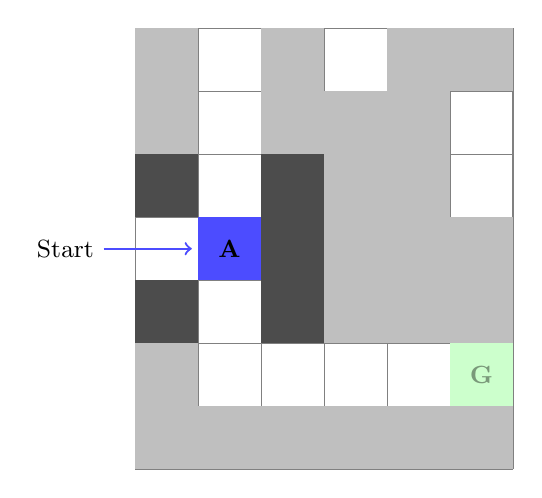
\begin{tikzpicture}[scale=0.8]
            \draw[step=1, gray, thin] (0,0) grid (6,7);

            % Agent at (1,3)-(2,4), surrounding tiles: x:0-3, y:2-5
            % Adjacent walls (full opacity)
            \fill[black!70] (2,3) rectangle (3,4);
            \fill[black!70] (2,4) rectangle (3,5);
            \fill[black!70] (0,2) rectangle (1,3);
            \fill[black!70] (0,4) rectangle (1,5);

            % Foggy walls - note: (0,3)-(1,4) is entrance, not wall
            \fill[black!25] (3,3) rectangle (6,4);
            \fill[black!25] (0,0) rectangle (1,2);
            \fill[black!25] (0,5) rectangle (1,7);
            \fill[black!25] (4,6) rectangle (6,7);
            \fill[black!25] (4,4) rectangle (5,6);
            \fill[black!25] (2,5) rectangle (3,7);  % extended wall
            \fill[black!25] (3,4) rectangle (4,6);  % extended inner wall

            % Fill blocks around the path
            \fill[black!25] (1,0) rectangle (6,1);  % row below path (foggy)
            \fill[black!70] (2,2) rectangle (3,3);  % adjacent to agent
            \fill[black!25] (3,2) rectangle (6,3);  % row above path (foggy)

            % Goal (foggy)
            \fill[green!20] (5,1) rectangle (6,2);
            \node[opacity=0.4] at (5.5,1.5) {\small \textbf{G}};

            \fill[blue!70] (1,3) rectangle (2,4);
            \node at (1.5,3.5) {\small \textbf{A}};
            % Start arrow
            \draw[->, thick, blue!70] (-0.5,3.5) -- (0.9,3.5);
            \node[left] at (-0.5,3.5) {\small Start};
        \end{tikzpicture}
    \end{center}
    \vspace{0.2cm}
    \begin{center}
        $Q((1,3), \text{down}) = ?$
    \end{center}
\end{frame}

%-----------------------------------------------
% Slide: Path Down - Step 2
%-----------------------------------------------
\begin{frame}{Bellman Equation: Path Down (Step 2)}
    \begin{center}
        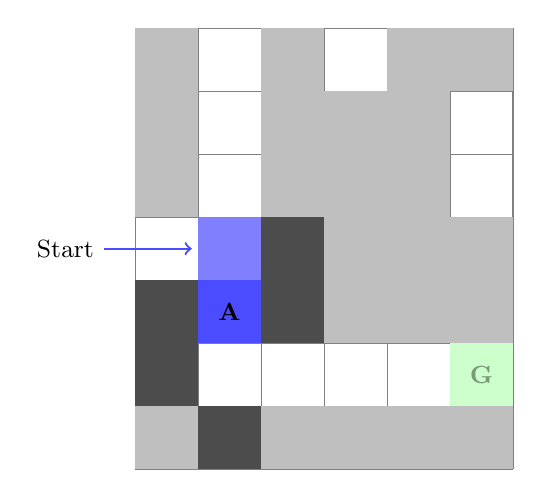
\begin{tikzpicture}[scale=0.8]
            \draw[step=1, gray, thin] (0,0) grid (6,7);

            % Agent at (1,2)-(2,3), surrounding tiles: x:0-3, y:1-4
            % Adjacent walls (full opacity)
            \fill[black!70] (2,3) rectangle (3,4);
            \fill[black!70] (0,1) rectangle (1,2);
            \fill[black!70] (0,2) rectangle (1,3);

            % Foggy walls - note: (0,3)-(1,4) is entrance, not wall
            \fill[black!25] (3,3) rectangle (6,4);
            \fill[black!25] (0,0) rectangle (1,1);
            \fill[black!25] (0,4) rectangle (1,7);
            \fill[black!25] (4,6) rectangle (6,7);
            \fill[black!25] (4,4) rectangle (5,6);
            \fill[black!25] (2,4) rectangle (3,7);  % extended wall
            \fill[black!25] (3,4) rectangle (4,6);  % extended inner wall

            % Fill blocks around the path
            \fill[black!70] (1,0) rectangle (2,1);  % adjacent to agent (below-left diagonal not quite, but 1,1 is adjacent)
            \fill[black!25] (2,0) rectangle (6,1);  % row below path (foggy)
            \fill[black!70] (2,2) rectangle (3,3);  % adjacent to agent
            \fill[black!25] (3,2) rectangle (6,3);  % row above path (foggy)

            % Goal (foggy)
            \fill[green!20] (5,1) rectangle (6,2);
            \node[opacity=0.4] at (5.5,1.5) {\small \textbf{G}};

            \fill[blue!50] (1,3) rectangle (2,4);
            \fill[blue!70] (1,2) rectangle (2,3);
            \node at (1.5,2.5) {\small \textbf{A}};
            % Start arrow
            \draw[->, thick, blue!70] (-0.5,3.5) -- (0.9,3.5);
            \node[left] at (-0.5,3.5) {\small Start};
        \end{tikzpicture}
    \end{center}
    \vspace{0.2cm}
    \begin{center}
        $Q((1,2), \text{down}) = ?$
    \end{center}
\end{frame}

%-----------------------------------------------
% Slide: Path Down - Step 3
%-----------------------------------------------
\begin{frame}{Bellman Equation: Path Down (Step 3)}
    \begin{center}
        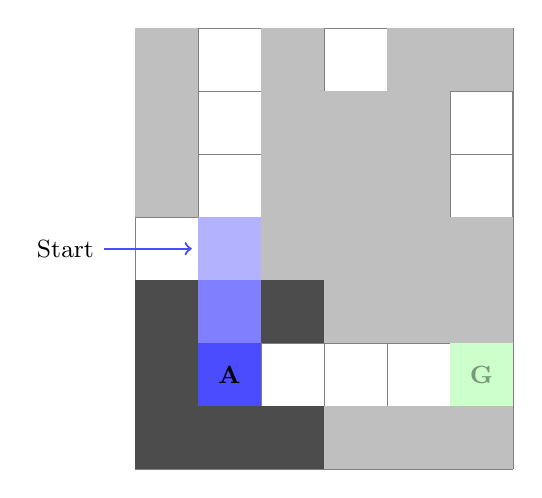
\begin{tikzpicture}[scale=0.8]
            \draw[step=1, gray, thin] (0,0) grid (6,7);

            % Agent at (1,1)-(2,2), surrounding tiles: x:0-3, y:0-3
            % Adjacent walls (full opacity)
            \fill[black!70] (0,0) rectangle (1,1);
            \fill[black!70] (0,1) rectangle (1,2);
            \fill[black!70] (0,2) rectangle (1,3);

            % Foggy walls - note: (0,3)-(1,4) is entrance, not wall
            \fill[black!25] (2,3) rectangle (6,4);
            \fill[black!25] (0,4) rectangle (1,7);
            \fill[black!25] (4,6) rectangle (6,7);
            \fill[black!25] (4,4) rectangle (5,6);
            \fill[black!25] (2,4) rectangle (3,7);  % extended wall
            \fill[black!25] (3,4) rectangle (4,6);  % extended inner wall

            % Fill blocks around the path
            \fill[black!70] (1,0) rectangle (2,1);  % adjacent to agent
            \fill[black!70] (2,0) rectangle (3,1);  % adjacent to agent
            \fill[black!25] (3,0) rectangle (6,1);  % row below path (foggy)
            \fill[black!70] (2,2) rectangle (3,3);  % adjacent to agent
            \fill[black!25] (3,2) rectangle (6,3);  % row above path (foggy)

            % Goal (foggy)
            \fill[green!20] (5,1) rectangle (6,2);
            \node[opacity=0.4] at (5.5,1.5) {\small \textbf{G}};

            \fill[blue!30] (1,3) rectangle (2,4);
            \fill[blue!50] (1,2) rectangle (2,3);
            \fill[blue!70] (1,1) rectangle (2,2);
            \node at (1.5,1.5) {\small \textbf{A}};
            % Start arrow
            \draw[->, thick, blue!70] (-0.5,3.5) -- (0.9,3.5);
            \node[left] at (-0.5,3.5) {\small Start};
        \end{tikzpicture}
    \end{center}
    \vspace{0.2cm}
    \begin{center}
        $Q((1,1), \text{right}) = ?$
    \end{center}
\end{frame}

%-----------------------------------------------
% Slide: Path Down - Step 4
%-----------------------------------------------
\begin{frame}{Bellman Equation: Path Down (Step 4)}
    \begin{center}
        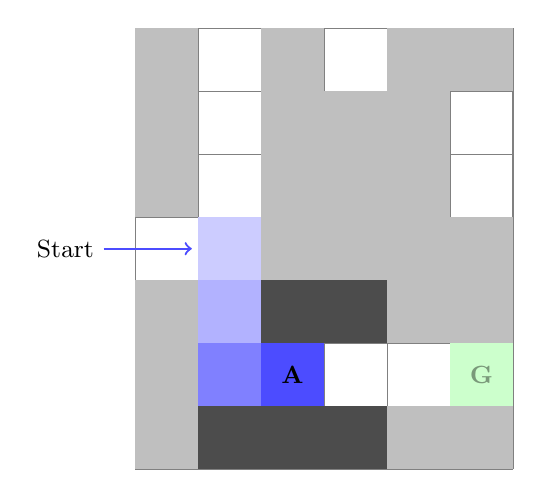
\begin{tikzpicture}[scale=0.8]
            \draw[step=1, gray, thin] (0,0) grid (6,7);

            % Agent at (2,1)-(3,2), surrounding tiles: x:1-4, y:0-3
            % Adjacent walls (full opacity) - none in this area

            % Foggy walls - note: (0,3)-(1,4) is entrance, not wall
            \fill[black!25] (2,3) rectangle (6,4);
            \fill[black!25] (0,0) rectangle (1,3);
            \fill[black!25] (0,4) rectangle (1,7);
            \fill[black!25] (4,6) rectangle (6,7);
            \fill[black!25] (4,4) rectangle (5,6);
            \fill[black!25] (2,4) rectangle (3,7);  % extended wall
            \fill[black!25] (3,4) rectangle (4,6);  % extended inner wall

            % Fill blocks around the path
            \fill[black!70] (1,0) rectangle (2,1);  % adjacent to agent
            \fill[black!70] (2,0) rectangle (3,1);  % adjacent to agent
            \fill[black!70] (3,0) rectangle (4,1);  % adjacent to agent
            \fill[black!25] (4,0) rectangle (6,1);  % row below path (foggy)
            \fill[black!70] (2,2) rectangle (3,3);  % adjacent to agent
            \fill[black!70] (3,2) rectangle (4,3);  % adjacent to agent
            \fill[black!25] (4,2) rectangle (6,3);  % row above path (foggy)

            % Goal (foggy)
            \fill[green!20] (5,1) rectangle (6,2);
            \node[opacity=0.4] at (5.5,1.5) {\small \textbf{G}};

            \fill[blue!20] (1,3) rectangle (2,4);
            \fill[blue!30] (1,2) rectangle (2,3);
            \fill[blue!50] (1,1) rectangle (2,2);
            \fill[blue!70] (2,1) rectangle (3,2);
            \node at (2.5,1.5) {\small \textbf{A}};
            % Start arrow
            \draw[->, thick, blue!70] (-0.5,3.5) -- (0.9,3.5);
            \node[left] at (-0.5,3.5) {\small Start};
        \end{tikzpicture}
    \end{center}
    \vspace{0.2cm}
    \begin{center}
        $Q((2,1), \text{right}) = ?$
    \end{center}
\end{frame}

%-----------------------------------------------
% Slide: Path Down - Step 5
%-----------------------------------------------
\begin{frame}{Bellman Equation: Path Down (Step 5)}
    \begin{center}
        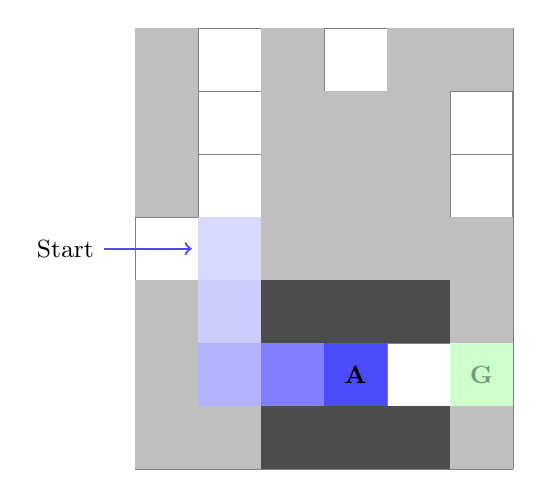
\begin{tikzpicture}[scale=0.8]
            \draw[step=1, gray, thin] (0,0) grid (6,7);

            % Agent at (3,1)-(4,2), surrounding tiles: x:2-5, y:0-3
            % Adjacent walls (full opacity) - none in this area

            % Foggy walls - note: (0,3)-(1,4) is entrance, not wall
            \fill[black!25] (2,3) rectangle (6,4);
            \fill[black!25] (0,0) rectangle (1,3);
            \fill[black!25] (0,4) rectangle (1,7);
            \fill[black!25] (4,6) rectangle (6,7);
            \fill[black!25] (4,4) rectangle (5,6);
            \fill[black!25] (2,4) rectangle (3,7);  % extended wall
            \fill[black!25] (3,4) rectangle (4,6);  % extended inner wall

            % Fill blocks around the path
            \fill[black!25] (1,0) rectangle (2,1);  % row below path (foggy)
            \fill[black!70] (2,0) rectangle (3,1);  % adjacent to agent
            \fill[black!70] (3,0) rectangle (4,1);  % adjacent to agent
            \fill[black!70] (4,0) rectangle (5,1);  % adjacent to agent
            \fill[black!25] (5,0) rectangle (6,1);  % row below path (foggy)
            \fill[black!70] (2,2) rectangle (3,3);  % adjacent to agent
            \fill[black!70] (3,2) rectangle (4,3);  % adjacent to agent
            \fill[black!70] (4,2) rectangle (5,3);  % adjacent to agent
            \fill[black!25] (5,2) rectangle (6,3);  % row above path (foggy)

            % Goal (foggy)
            \fill[green!20] (5,1) rectangle (6,2);
            \node[opacity=0.4] at (5.5,1.5) {\small \textbf{G}};

            \fill[blue!15] (1,3) rectangle (2,4);
            \fill[blue!20] (1,2) rectangle (2,3);
            \fill[blue!30] (1,1) rectangle (2,2);
            \fill[blue!50] (2,1) rectangle (3,2);
            \fill[blue!70] (3,1) rectangle (4,2);
            \node at (3.5,1.5) {\small \textbf{A}};
            % Start arrow
            \draw[->, thick, blue!70] (-0.5,3.5) -- (0.9,3.5);
            \node[left] at (-0.5,3.5) {\small Start};
        \end{tikzpicture}
    \end{center}
    \vspace{0.2cm}
    \begin{center}
        $Q((3,1), \text{right}) = ?$
    \end{center}
\end{frame}

%-----------------------------------------------
% Slide: Path Down - Step 6
%-----------------------------------------------
\begin{frame}{Bellman Equation: Path Down (Step 6)}
    \begin{center}
        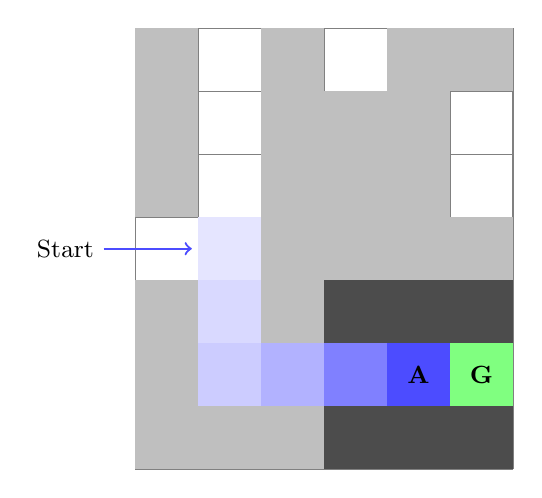
\begin{tikzpicture}[scale=0.8]
            \draw[step=1, gray, thin] (0,0) grid (6,7);

            % Agent at (4,1)-(5,2), surrounding tiles: x:3-6, y:0-3
            % Adjacent walls (full opacity) - none in this area

            % Foggy walls - note: (0,3)-(1,4) is entrance, not wall
            \fill[black!25] (2,3) rectangle (6,4);
            \fill[black!25] (0,0) rectangle (1,3);
            \fill[black!25] (0,4) rectangle (1,7);
            \fill[black!25] (4,6) rectangle (6,7);
            \fill[black!25] (4,4) rectangle (5,6);
            \fill[black!25] (2,4) rectangle (3,7);  % extended wall
            \fill[black!25] (3,4) rectangle (4,6);  % extended inner wall

            % Fill blocks around the path
            \fill[black!25] (1,0) rectangle (3,1);  % row below path (foggy)
            \fill[black!70] (3,0) rectangle (4,1);  % adjacent to agent
            \fill[black!70] (4,0) rectangle (5,1);  % adjacent to agent
            \fill[black!70] (5,0) rectangle (6,1);  % adjacent to agent
            \fill[black!25] (2,2) rectangle (3,3);  % row above path (foggy)
            \fill[black!70] (3,2) rectangle (4,3);  % adjacent to agent
            \fill[black!70] (4,2) rectangle (5,3);  % adjacent to agent
            \fill[black!70] (5,2) rectangle (6,3);  % adjacent to agent

            % Goal (visible - adjacent to agent!)
            \fill[green!50] (5,1) rectangle (6,2);
            \node at (5.5,1.5) {\small \textbf{G}};

            \fill[blue!10] (1,3) rectangle (2,4);
            \fill[blue!15] (1,2) rectangle (2,3);
            \fill[blue!20] (1,1) rectangle (2,2);
            \fill[blue!30] (2,1) rectangle (3,2);
            \fill[blue!50] (3,1) rectangle (4,2);
            \fill[blue!70] (4,1) rectangle (5,2);
            \node at (4.5,1.5) {\small \textbf{A}};
            % Start arrow
            \draw[->, thick, blue!70] (-0.5,3.5) -- (0.9,3.5);
            \node[left] at (-0.5,3.5) {\small Start};
        \end{tikzpicture}
    \end{center}
    \vspace{0.2cm}
    \begin{center}
        $Q((4,1), \text{right}) = ?$
    \end{center}
\end{frame}

%-----------------------------------------------
% Slide: Path Down - Step 7 (Goal!)
%-----------------------------------------------
\begin{frame}{Bellman Equation: Path Down (Goal!)}
    \begin{center}
        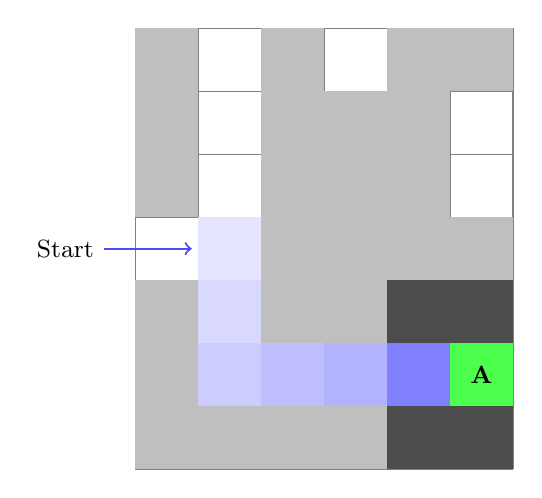
\begin{tikzpicture}[scale=0.8]
            \draw[step=1, gray, thin] (0,0) grid (6,7);

            % Agent at goal (5,1)-(6,2), surrounding tiles: x:4-6, y:0-3
            % Adjacent walls (full opacity) - none in this area

            % Foggy walls - note: (0,3)-(1,4) is entrance, not wall
            \fill[black!25] (2,3) rectangle (6,4);
            \fill[black!25] (0,0) rectangle (1,3);
            \fill[black!25] (0,4) rectangle (1,7);
            \fill[black!25] (4,6) rectangle (6,7);
            \fill[black!25] (4,4) rectangle (5,6);
            \fill[black!25] (2,4) rectangle (3,7);  % extended wall
            \fill[black!25] (3,4) rectangle (4,6);  % extended inner wall

            % Fill remaining empty blocks around the path
            \fill[black!25] (1,0) rectangle (4,1);  % row below path (foggy)
            \fill[black!70] (4,0) rectangle (5,1);  % adjacent to agent
            \fill[black!70] (5,0) rectangle (6,1);  % adjacent to agent
            \fill[black!25] (2,2) rectangle (4,3);  % row above path (foggy)
            \fill[black!70] (4,2) rectangle (5,3);  % adjacent to agent
            \fill[black!70] (5,2) rectangle (6,3);  % adjacent to agent

            \fill[blue!10] (1,3) rectangle (2,4);
            \fill[blue!15] (1,2) rectangle (2,3);
            \fill[blue!20] (1,1) rectangle (2,2);
            \fill[blue!25] (2,1) rectangle (3,2);
            \fill[blue!30] (3,1) rectangle (4,2);
            \fill[blue!50] (4,1) rectangle (5,2);
            \fill[green!70] (5,1) rectangle (6,2);
            \node at (5.5,1.5) {\small \textbf{A}};
            % Start arrow
            \draw[->, thick, blue!70] (-0.5,3.5) -- (0.9,3.5);
            \node[left] at (-0.5,3.5) {\small Start};
        \end{tikzpicture}
    \end{center}

    \vspace{0.3cm}
    \begin{center}
        {\color{green!50!black} Agent reaches the goal!}
    \end{center}
\end{frame}

%-----------------------------------------------
% SLIDE: Bellman Q-Value Calculations
%-----------------------------------------------
\begin{frame}{Bellman Equation: Q-Value Calculations}
    \begin{columns}[T]
        \begin{column}{0.48\textwidth}
            \centering
            {\color{red}\textbf{Path Up (Dead End)}}
            \vspace{0.2cm}

            \scriptsize
            \begin{tabular}{|c|c|c|c|}
                \hline
                \textbf{State} & \textbf{Action} & \textbf{R} & \textbf{Q(s,a)} \\
                \hline
                (1,3) & up & -0.01 & -0.01 \\
                (1,4) & up & -0.01 & -0.02 \\
                (1,5) & up & -0.01 & -0.03 \\
                (1,6) & right & -0.01 & -0.04 \\
                (2,6) & right & -0.01 & -0.05 \\
                (3,6) & down & -0.01 & -0.06 \\
                (3,5) & -- & -10 & \textbf{-10.06} \\
                \hline
            \end{tabular}

            \vspace{0.3cm}
            $Q(\text{Start}, \text{up}) = -10.06$
        \end{column}

        \begin{column}{0.48\textwidth}
            \centering
            {\color{green!50!black}\textbf{Path Down (Goal)}}
            \vspace{0.2cm}

            \scriptsize
            \begin{tabular}{|c|c|c|c|}
                \hline
                \textbf{State} & \textbf{Action} & \textbf{R} & \textbf{Q(s,a)} \\
                \hline
                (1,3) & down & -0.01 & -0.01 \\
                (1,2) & down & -0.01 & -0.02 \\
                (1,1) & right & -0.01 & -0.03 \\
                (2,1) & right & -0.01 & -0.04 \\
                (3,1) & right & -0.01 & -0.05 \\
                (4,1) & right & -0.01 & -0.06 \\
                (5,1) & -- & +10 & \textbf{+9.94} \\
                \hline
            \end{tabular}

            \vspace{0.3cm}
            $Q(\text{Start}, \text{down}) = +9.94$
        \end{column}
    \end{columns}

    \vspace{0.5cm}
    \begin{center}
        \fbox{Agent learns: \textbf{down} is better because $Q(\text{down}) > Q(\text{up})$}
    \end{center}
\end{frame}

%-----------------------------------------------
% SECTION: PRESENTER B - Algorithms & Implementation
%-----------------------------------------------

%-----------------------------------------------
% SLIDE: Problems with Raw Rewards
%-----------------------------------------------
\begin{frame}{Problems with the Current Reward System}
    \begin{center}
        \textit{Why not just use raw rewards?}
    \end{center}
\end{frame}

%-----------------------------------------------
% SLIDE: Raw Rewards Example
%-----------------------------------------------
\begin{frame}{Problems with the Current Reward System}
    \begin{columns}[T]
        \begin{column}{0.48\textwidth}
            \centering
            \textbf{Scenario A}

            \vspace{0.3cm}
            \begin{tabular}{|c|c|}
                \hline
                Action & Reward \\
                \hline
                Left & -5 \\
                Forward & 0 \\
                Right & +5 \\
                \hline
            \end{tabular}

            \vspace{0.3cm}
            Best: \textbf{Right} (+5)
        \end{column}

        \begin{column}{0.48\textwidth}
            \centering
            \textbf{Scenario B}

            \vspace{0.3cm}
            \begin{tabular}{|c|c|}
                \hline
                Action & Reward \\
                \hline
                Left & +95 \\
                Forward & +100 \\
                Right & +105 \\
                \hline
            \end{tabular}

            \vspace{0.3cm}
            Best: \textbf{Right} (+105)
        \end{column}
    \end{columns}

    \vspace{0.5cm}
    \begin{center}
        Same decision, but raw values are very different!
    \end{center}
\end{frame}

%-----------------------------------------------
% SLIDE: Credit Assignment Problem - Question
%-----------------------------------------------
\begin{frame}{The Credit Assignment Problem}
    \begin{center}
        \textit{Which action should the agent take?}
    \end{center}

    \vspace{0.5cm}
    \begin{center}
        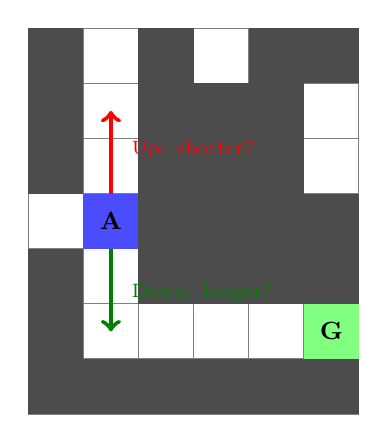
\begin{tikzpicture}[scale=0.7]
            % Grid
            \draw[step=1, gray, thin] (0,0) grid (6,7);
            % Walls - same maze shape as Bellman diagrams
            \fill[black!70] (2,3) rectangle (6,4);
            \fill[black!70] (0,0) rectangle (1,3);
            \fill[black!70] (0,4) rectangle (1,7);
            \fill[black!70] (4,6) rectangle (6,7);
            \fill[black!70] (4,4) rectangle (5,6);
            \fill[black!70] (2,4) rectangle (3,7);  % extended wall blocking upper path
            \fill[black!70] (3,4) rectangle (4,6);  % extended inner wall
            % Fill blocks around the path
            \fill[black!70] (1,0) rectangle (6,1);  % row below path
            \fill[black!70] (2,2) rectangle (6,3);  % row above path
            % Goal
            \fill[green!50] (5,1) rectangle (6,2);
            \node at (5.5,1.5) {\small \textbf{G}};
            % Agent
            \fill[blue!70] (1,3) rectangle (2,4);
            \node at (1.5,3.5) {\small \textbf{A}};
            % Arrows with initial rewards
            \draw[->, red, ultra thick] (1.5,4) -- (1.5,5.5);
            \node[right, red] at (1.7,4.8) {\scriptsize Up: shorter?};
            \draw[->, green!50!black, ultra thick] (1.5,3) -- (1.5,1.5);
            \node[right, green!50!black] at (1.7,2.2) {\scriptsize Down: longer?};
        \end{tikzpicture}
    \end{center}
\end{frame}

%-----------------------------------------------
% SLIDE: Credit Assignment Problem - Explanation
%-----------------------------------------------
\begin{frame}{The Credit Assignment Problem}
    \begin{columns}[T]
        \begin{column}{0.55\textwidth}
            \begin{center}
                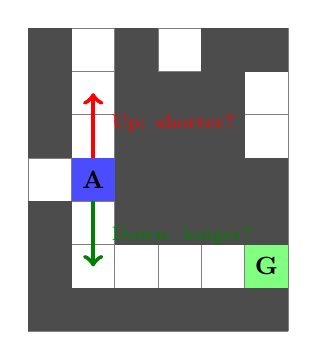
\begin{tikzpicture}[scale=0.55]
                    % Grid
                    \draw[step=1, gray, thin] (0,0) grid (6,7);
                    % Walls - same maze shape as Bellman diagrams
                    \fill[black!70] (2,3) rectangle (6,4);
                    \fill[black!70] (0,0) rectangle (1,3);
                    \fill[black!70] (0,4) rectangle (1,7);
                    \fill[black!70] (4,6) rectangle (6,7);
                    \fill[black!70] (4,4) rectangle (5,6);
                    \fill[black!70] (2,4) rectangle (3,7);  % extended wall blocking upper path
                    \fill[black!70] (3,4) rectangle (4,6);  % extended inner wall
                    % Fill blocks around the path
                    \fill[black!70] (1,0) rectangle (6,1);  % row below path
                    \fill[black!70] (2,2) rectangle (6,3);  % row above path
                    % Goal
                    \fill[green!50] (5,1) rectangle (6,2);
                    \node at (5.5,1.5) {\small \textbf{G}};
                    % Agent
                    \fill[blue!70] (1,3) rectangle (2,4);
                    \node at (1.5,3.5) {\small \textbf{A}};
                    % Arrows with initial rewards
                    \draw[->, red, ultra thick] (1.5,4) -- (1.5,5.5);
                    \node[right, red] at (1.7,4.8) {\scriptsize Up: shorter?};
                    \draw[->, green!50!black, ultra thick] (1.5,3) -- (1.5,1.5);
                    \node[right, green!50!black] at (1.7,2.2) {\scriptsize Down: longer?};
                \end{tikzpicture}
            \end{center}
        \end{column}

        \begin{column}{0.42\textwidth}
            \textbf{Initial estimate:}
            \begin{itemize}
                \item Up looks shorter
                \item Down looks longer
            \end{itemize}

            \vspace{0.3cm}
            \textbf{But reality:}
            \begin{itemize}
                \item Up $\rightarrow$ {\color{red}dead end!}
                \item Down $\rightarrow$ {\color{green!50!black}reaches goal}
            \end{itemize}

            \vspace{0.3cm}
            \textbf{Problem:}\\
            How to assign credit to early actions based on later outcomes?
        \end{column}
    \end{columns}

    \vspace{0.3cm}
    \begin{center}
        \fbox{TD Learning propagates rewards backwards to solve this}
    \end{center}
\end{frame}

%-----------------------------------------------
% SLIDE: Temporal Difference Learning
%-----------------------------------------------
\begin{frame}{Temporal Difference (TD) Learning}
    \begin{columns}[T]
        \begin{column}{0.48\textwidth}
            \centering
            \textbf{1. Q estimates (3 states)}
            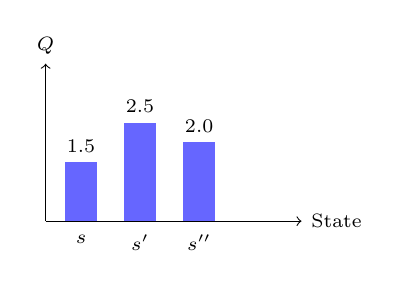
\begin{tikzpicture}[scale=0.5]
                % Axes (same width as graph 3)
                \draw[->] (0,0) -- (6.5,0) node[right] {\scriptsize State};
                \draw[->] (0,0) -- (0,4) node[above] {\scriptsize $Q$};

                % Q values as bars
                \fill[blue!60] (0.5,0) rectangle (1.3,1.5);
                \fill[blue!60] (2,0) rectangle (2.8,2.5);
                \fill[blue!60] (3.5,0) rectangle (4.3,2);

                % Values on bars
                \node[above] at (0.9,1.5) {\scriptsize 1.5};
                \node[above] at (2.4,2.5) {\scriptsize 2.5};
                \node[above] at (3.9,2) {\scriptsize 2.0};

                % Labels
                \node[below] at (0.9,-0.1) {\scriptsize $s$};
                \node[below] at (2.4,-0.1) {\scriptsize $s'$};
                \node[below] at (3.9,-0.1) {\scriptsize $s''$};
            \end{tikzpicture}

            \vspace{0.5cm}
            \textbf{3. New state $s'''$ arrives}
            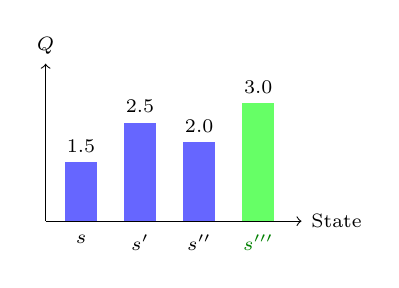
\begin{tikzpicture}[scale=0.5]
                % Axes
                \draw[->] (0,0) -- (6.5,0) node[right] {\scriptsize State};
                \draw[->] (0,0) -- (0,4) node[above] {\scriptsize $Q$};

                % Q values as bars
                \fill[blue!60] (0.5,0) rectangle (1.3,1.5);
                \fill[blue!60] (2,0) rectangle (2.8,2.5);
                \fill[blue!60] (3.5,0) rectangle (4.3,2);
                \fill[green!60] (5,0) rectangle (5.8,3);

                % Values on bars
                \node[above] at (0.9,1.5) {\scriptsize 1.5};
                \node[above] at (2.4,2.5) {\scriptsize 2.5};
                \node[above] at (3.9,2) {\scriptsize 2.0};
                \node[above] at (5.4,3) {\scriptsize 3.0};

                % Labels
                \node[below] at (0.9,-0.1) {\scriptsize $s$};
                \node[below] at (2.4,-0.1) {\scriptsize $s'$};
                \node[below] at (3.9,-0.1) {\scriptsize $s''$};
                \node[below, green!50!black] at (5.4,-0.1) {\scriptsize $s'''$};
            \end{tikzpicture}
        \end{column}

        \begin{column}{0.48\textwidth}
            \centering
            \textbf{2. TD errors (normalized)}
            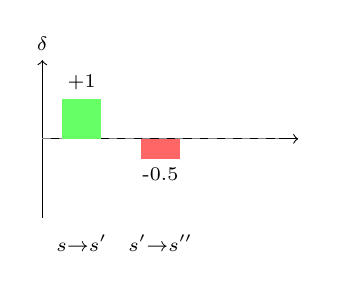
\begin{tikzpicture}[scale=0.5]
                % Axes (same height as Q graphs: -2 to 2 = 4 units)
                \draw[->] (0,0) -- (6.5,0) node[right] {\scriptsize};
                \draw[->] (0,-2) -- (0,2) node[above] {\scriptsize $\delta$};
                \draw[gray, dashed] (0,0) -- (6,0);

                % TD error bars (2.5-1.5=+1, 2.0-2.5=-0.5)
                \fill[green!60] (0.5,0) rectangle (1.5,1);
                \fill[red!60] (2.5,0) rectangle (3.5,-0.5);

                % Labels
                \node[below] at (1,-2.2) {\scriptsize $s{\to}s'$};
                \node[below] at (3,-2.2) {\scriptsize $s'{\to}s''$};

                % Values
                \node[above] at (1,1) {\scriptsize +1};
                \node[below] at (3,-0.5) {\scriptsize -0.5};
            \end{tikzpicture}

            \vspace{0.5cm}
            \textbf{4. TD errors change!}
            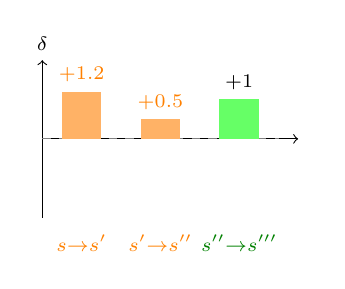
\begin{tikzpicture}[scale=0.5]
                % Axes (same height as Q graphs: -2 to 2 = 4 units)
                \draw[->] (0,0) -- (6.5,0) node[right] {\scriptsize};
                \draw[->] (0,-2) -- (0,2) node[above] {\scriptsize $\delta$};
                \draw[gray, dashed] (0,0) -- (6,0);

                % TD error bars - all change due to propagation
                \fill[orange!60] (0.5,0) rectangle (1.5,1.2);
                \fill[orange!60] (2.5,0) rectangle (3.5,0.5);
                \fill[green!60] (4.5,0) rectangle (5.5,1);

                % Labels
                \node[below, orange] at (1,-2.2) {\scriptsize $s{\to}s'$};
                \node[below, orange] at (3,-2.2) {\scriptsize $s'{\to}s''$};
                \node[below, green!50!black] at (5,-2.2) {\scriptsize $s''{\to}s'''$};

                % Values (propagated changes)
                \node[above, orange] at (1,1.2) {\scriptsize +1.2};
                \node[above, orange] at (3,0.5) {\scriptsize +0.5};
                \node[above] at (5,1) {\scriptsize +1};
            \end{tikzpicture}
        \end{column}
    \end{columns}

    \vspace{0.3cm}
    \begin{center}
        \fbox{TD uses \textbf{difference} $\delta = Q(s') - Q(s)$ as learning signal, not raw values}
    \end{center}
\end{frame}

%-----------------------------------------------
% SLIDE: Exploration vs. Exploitation
%-----------------------------------------------
\begin{frame}{Exploration vs. Exploitation}
    \begin{center}
        \textit{The agent found food going down. Should it always go down?}
    \end{center}

    \vspace{0.5cm}
    \begin{columns}[T]
        \begin{column}{0.48\textwidth}
            \centering
            \textbf{Exploration}

            \vspace{0.3cm}
            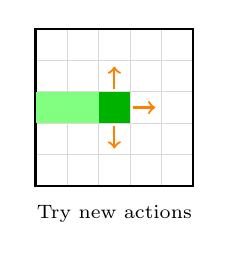
\begin{tikzpicture}[scale=0.4]
                % Grid
                \draw[gray!30] (0,0) grid (5,5);
                \draw[black, thick] (0,0) rectangle (5,5);
                % Snake body (left to right)
                \fill[green!50] (0,2) rectangle (1,3);
                \fill[green!50] (1,2) rectangle (2,3);
                % Snake head
                \fill[green!70!black] (2,2) rectangle (3,3);
                % Arrows in multiple directions
                \draw[->, thick, orange] (2.5,3.1) -- (2.5,3.8);
                \draw[->, thick, orange] (3.1,2.5) -- (3.8,2.5);
                \draw[->, thick, orange] (2.5,1.9) -- (2.5,1.2);
                \node[below] at (2.5,-0.3) {\scriptsize Try new actions};
            \end{tikzpicture}

            \vspace{0.3cm}
            Discover better strategies
        \end{column}

        \begin{column}{0.48\textwidth}
            \centering
            \textbf{Exploitation}

            \vspace{0.3cm}
            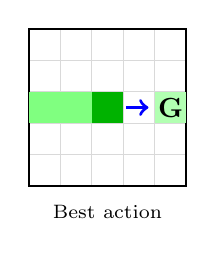
\begin{tikzpicture}[scale=0.4]
                % Grid
                \draw[gray!30] (0,0) grid (5,5);
                \draw[black, thick] (0,0) rectangle (5,5);
                % Snake body (left to right)
                \fill[green!50] (0,2) rectangle (1,3);
                \fill[green!50] (1,2) rectangle (2,3);
                % Snake head
                \fill[green!70!black] (2,2) rectangle (3,3);
                % Goal to the right
                \fill[green!30] (4,2) rectangle (5,3);
                \node at (4.5,2.5) {\textbf{G}};
                % Arrow right (best known action)
                \draw[->, very thick, blue] (3.1,2.5) -- (3.8,2.5);
                \node[below] at (2.5,-0.3) {\scriptsize Best action};
            \end{tikzpicture}

            \vspace{0.3cm}
            Use current knowledge
        \end{column}
    \end{columns}

    \vspace{0.5cm}
    \begin{center}
        \fbox{Balance is key: too much exploration = slow; too little = suboptimal}
    \end{center}
\end{frame}

%-----------------------------------------------
% SLIDE: Epsilon-Greedy Strategy
%-----------------------------------------------
\begin{frame}{$\epsilon$-Greedy Strategy \hfill {\color{red}\textbf{TODO}}}
    \begin{columns}[T]
        \begin{column}{0.48\textwidth}
            \centering
            \textbf{High $\epsilon$ = 0.75} (Early training)

            \vspace{0.3cm}
            $\pi(a|s)$:
            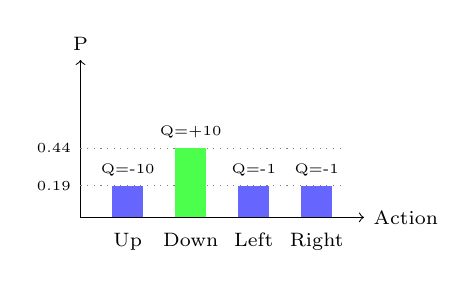
\begin{tikzpicture}[scale=0.8]
                % Axes
                \draw[->] (0,0) -- (4.5,0) node[right] {\scriptsize Action};
                \draw[->] (0,0) -- (0,2.5) node[above] {\scriptsize P};
                % Y-axis labels
                \node[left] at (0,0.5) {\tiny 0.19};
                \node[left] at (0,1.1) {\tiny 0.44};
                \draw[gray, dotted] (0,0.5) -- (4.2,0.5);
                \draw[gray, dotted] (0,1.1) -- (4.2,1.1);
                % Bars - 75% random (18.75% each) + 25% best
                % best gets 25% + 75%/4 = 43.75%, others get 75%/4 = 18.75%
                \fill[blue!60] (0.5,0) rectangle (1,0.5);
                \fill[green!70] (1.5,0) rectangle (2,1.1);
                \fill[blue!60] (2.5,0) rectangle (3,0.5);
                \fill[blue!60] (3.5,0) rectangle (4,0.5);
                % Labels
                \node[below] at (0.75,-0.1) {\scriptsize Up};
                \node[below] at (1.75,-0.1) {\scriptsize Down};
                \node[below] at (2.75,-0.1) {\scriptsize Left};
                \node[below] at (3.75,-0.1) {\scriptsize Right};
                % Rewards above bars
                \node[above] at (0.75,0.5) {\tiny Q=-10};
                \node[above] at (1.75,1.1) {\tiny Q=+10};
                \node[above] at (2.75,0.5) {\tiny Q=-1};
                \node[above] at (3.75,0.5) {\tiny Q=-1};
            \end{tikzpicture}

            \vspace{0.2cm}
            {\small More exploration}
        \end{column}

        \begin{column}{0.48\textwidth}
            \centering
            \textbf{Low $\epsilon$ = 0.25} (Late training)

            \vspace{0.3cm}
            $\pi(a|s)$:
            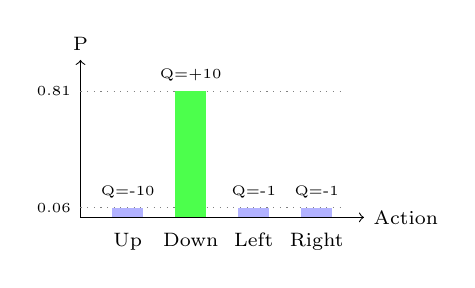
\begin{tikzpicture}[scale=0.8]
                % Axes
                \draw[->] (0,0) -- (4.5,0) node[right] {\scriptsize Action};
                \draw[->] (0,0) -- (0,2.5) node[above] {\scriptsize P};
                % Y-axis labels
                \node[left] at (0,0.15) {\tiny 0.06};
                \node[left] at (0,2) {\tiny 0.81};
                \draw[gray, dotted] (0,0.15) -- (4.2,0.15);
                \draw[gray, dotted] (0,2) -- (4.2,2);
                % Bars - best gets 75% + 25%/4 = 81.25%, others get 25%/4 = 6.25%
                \fill[blue!30] (0.5,0) rectangle (1,0.15);
                \fill[green!70] (1.5,0) rectangle (2,2);
                \fill[blue!30] (2.5,0) rectangle (3,0.15);
                \fill[blue!30] (3.5,0) rectangle (4,0.15);
                % Labels
                \node[below] at (0.75,-0.1) {\scriptsize Up};
                \node[below] at (1.75,-0.1) {\scriptsize Down};
                \node[below] at (2.75,-0.1) {\scriptsize Left};
                \node[below] at (3.75,-0.1) {\scriptsize Right};
                % Rewards above bars
                \node[above] at (0.75,0.15) {\tiny Q=-10};
                \node[above] at (1.75,2) {\tiny Q=+10};
                \node[above] at (2.75,0.15) {\tiny Q=-1};
                \node[above] at (3.75,0.15) {\tiny Q=-1};
            \end{tikzpicture}

            \vspace{0.2cm}
            {\small Best action dominates}
        \end{column}
    \end{columns}

    \vspace{0.5cm}
    \begin{center}
        \fbox{$\epsilon$: choose randomly $\epsilon$\% of the time}
    \end{center}
\end{frame}

%-----------------------------------------------
% SLIDE: Learning Q (Action-Value)
%-----------------------------------------------
\begin{frame}{Learning Q (Action-Value)}
    \textbf{SARSA} (On-policy) -- {\small Uses the action $a'$ actually taken in $s'$}
    \[
    Q(s,a) \leftarrow Q(s,a) + \alpha \left[ r + \gamma Q(s', a') - Q(s,a) \right]
    \]

    \vspace{0.2cm}
    \textbf{Expected SARSA} -- {\small Uses expected value over all actions in $s'$}
    \[
    Q(s,a) \leftarrow Q(s,a) + \alpha \left[ r + \gamma \sum_{a'} \pi(a'|s') Q(s', a') - Q(s,a) \right]
    \]

    \vspace{0.2cm}
    \textbf{Q-Learning} (Off-policy) -- {\small Uses the best action in $s'$ (regardless of policy)}
    \[
    Q(s,a) \leftarrow Q(s,a) + \alpha \left[ r + \gamma \max_{a'} Q(s', a') - Q(s,a) \right]
    \]
\end{frame}

%-----------------------------------------------
% SLIDE: Learning V (State-Value)
%-----------------------------------------------
\begin{frame}{Learning V (State-Value)}
    \textbf{TD(0)} -- One-step temporal difference
    \[
    V(s) \leftarrow V(s) + \alpha \left[ r + \gamma V(s') - V(s) \right]
    \]

    \vspace{0.5cm}
    \textbf{TD($\lambda$)} -- Multi-step with eligibility traces
    \[
    V(s) \leftarrow V(s) + \alpha \delta_t e_t(s)
    \]
    {\small where $e_t(s)$ is the eligibility trace and $\lambda \in [0,1]$ controls the trace decay}

    \vspace{0.5cm}
    \textbf{Monte Carlo}
    \[
    V(s) \leftarrow V(s) + \alpha \left[ G_t - V(s) \right]
    \]
    {\small $G_t$ = total return from state $s$ (wait until episode ends)}
\end{frame}

%-----------------------------------------------
% SLIDE: DQN Family
%-----------------------------------------------
\begin{frame}{Value-Based Methods: DQN Family}
    \begin{itemize}
        \item \textbf{DQN (Deep Q-Network)} -- Neural network approximates Q(s,a); experience replay; target network
        \item \textbf{Double DQN} -- Reduces overestimation bias; separate networks for selection \& evaluation
        \item \textbf{Dueling DQN} -- Separates value \& advantage: $Q(s,a) = V(s) + A(s,a)$
        \item \textbf{Noisy DQN} -- Learned exploration; no $\epsilon$-greedy needed
        \item \textbf{PER DQN} -- Prioritized experience replay; learn more from important transitions
    \end{itemize}
\end{frame}

%-----------------------------------------------
% SLIDE: Experience Replay
%-----------------------------------------------
\begin{frame}{Experience Replay}
    \vspace{0.3cm}
    \begin{columns}[T]
        \begin{column}{0.48\textwidth}
            \centering
            \textbf{Without Replay}

            \vspace{0.3cm}
            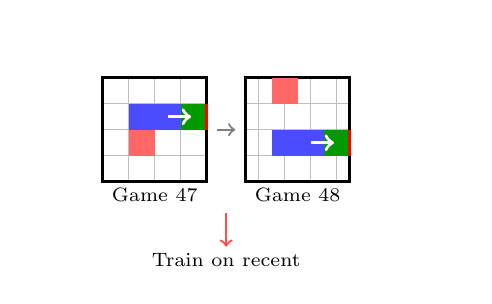
\begin{tikzpicture}[scale=0.33]
                % Invisible nodes to match height of right diagram
                \node at (5.5,5.2) {\scriptsize \phantom{Memory Buffer (stores diverse experiences)}};
                \path (0,-3) -- (0,-3); % match bottom of right diagram

                % Game 47: Snake hitting right wall
                \draw[gray!50] (0,0) grid (4,4);
                \draw[black, very thick] (0,0) rectangle (4,4);
                \fill[red!60] (1,1) rectangle (2,2);  % food (ignored)
                \fill[blue!70] (1,2) rectangle (2,3);  % body
                \fill[blue!70] (2,2) rectangle (3,3);  % body
                \fill[green!60!black] (3,2) rectangle (4,3);  % head at wall
                \draw[->, very thick, white] (2.5,2.5) -- (3.4,2.5);  % direction arrow
                \draw[red, very thick] (4,2) -- (4,3);  % collision indicator
                \node at (2,-0.5) {\scriptsize Game 47};

                % Arrow between games
                \draw[->, thick, gray] (4.4,2) -- (5.1,2);

                % Game 48: Snake hitting right wall again (similar)
                \draw[gray!50] (5.5,0) grid (9.5,4);
                \draw[black, very thick] (5.5,0) rectangle (9.5,4);
                \fill[red!60] (6.5,3) rectangle (7.5,4);  % food (ignored)
                \fill[blue!70] (6.5,1) rectangle (7.5,2);  % body
                \fill[blue!70] (7.5,1) rectangle (8.5,2);  % body
                \fill[green!60!black] (8.5,1) rectangle (9.5,2);  % head at wall
                \draw[->, very thick, white] (8,1.5) -- (8.9,1.5);  % direction arrow
                \draw[red, very thick] (9.5,1) -- (9.5,2);  % collision indicator
                \node at (7.5,-0.5) {\scriptsize Game 48};

                % Arrow to neural network
                \draw[->, thick, red!70] (4.75,-1.2) -- (4.75,-2.5);
                \node at (4.75,-3) {\scriptsize Train on recent};
            \end{tikzpicture}

            \vspace{0.5cm}
            \begin{minipage}[t][2.5cm][t]{\linewidth}
                \centering
                {\color{red} \textbf{Problem:}}\\[0.2cm]
                Agent keeps dying to walls\\
                $\rightarrow$ Only learns ``avoid walls''\\
                $\rightarrow$ Forgets how to get food!
            \end{minipage}
        \end{column}

        \begin{column}{0.48\textwidth}
            \centering
            \textbf{With Replay}

            \vspace{0.3cm}
            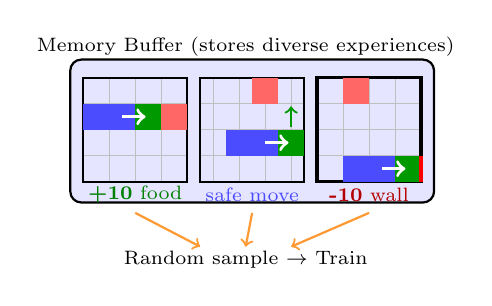
\begin{tikzpicture}[scale=0.33]
                % Memory buffer with mixed experiences
                \draw[thick, fill=blue!10, rounded corners] (-0.5,-0.8) rectangle (13.5,4.7);
                \node at (6.25,5.2) {\scriptsize Memory Buffer (stores diverse experiences)};

                % Experience 1: Snake eating food (positive reward)
                \draw[gray!50] (0,0) grid (4,4);
                \draw[black, thick] (0,0) rectangle (4,4);
                \fill[blue!70] (0,2) rectangle (1,3);  % body
                \fill[blue!70] (1,2) rectangle (2,3);  % body
                \fill[green!60!black] (2,2) rectangle (3,3);  % head
                \fill[red!60] (3,2) rectangle (4,3);  % food (about to eat)
                \draw[->, very thick, white] (1.5,2.5) -- (2.4,2.5);  % direction arrow
                \node[green!50!black] at (2,-0.5) {\scriptsize \textbf{+10} food};

                % Experience 2: Snake avoiding wall (learned behavior)
                \draw[gray!50] (4.5,0) grid (8.5,4);
                \draw[black, thick] (4.5,0) rectangle (8.5,4);
                \fill[blue!70] (5.5,1) rectangle (6.5,2);  % body
                \fill[blue!70] (6.5,1) rectangle (7.5,2);  % body
                \fill[green!60!black] (7.5,1) rectangle (8.5,2);  % head
                \fill[red!60] (6.5,3) rectangle (7.5,4);  % food elsewhere
                \draw[->, very thick, white] (7,1.5) -- (7.9,1.5);  % direction arrow
                \draw[->, thick, green!60!black] (8,2.1) -- (8,2.9);  % turning up
                \node[blue!70] at (6.5,-0.5) {\scriptsize safe move};

                % Experience 3: Snake hitting wall (negative reward)
                \draw[gray!50] (9,0) grid (13,4);
                \draw[black, very thick] (9,0) rectangle (13,4);
                \fill[red!60] (10,3) rectangle (11,4);  % food (missed)
                \fill[blue!70] (10,0) rectangle (11,1);  % body
                \fill[blue!70] (11,0) rectangle (12,1);  % body
                \fill[green!60!black] (12,0) rectangle (13,1);  % head at wall
                \draw[->, very thick, white] (11.5,0.5) -- (12.4,0.5);  % direction arrow
                \draw[red, very thick] (13,0) -- (13,1);  % collision
                \node[red!70!black] at (11,-0.5) {\scriptsize \textbf{-10} wall};
                % Right margin
                \path (14,0) -- (14,0);

                % Random sampling arrows
                \draw[->, thick, orange!80] (2,-1.2) -- (4.5,-2.5);
                \draw[->, thick, orange!80] (6.5,-1.2) -- (6.25,-2.5);
                \draw[->, thick, orange!80] (11,-1.2) -- (8,-2.5);
                \node at (6.25,-3) {\scriptsize Random sample $\rightarrow$ Train};
            \end{tikzpicture}

            \vspace{0.5cm}
            \begin{minipage}[t][2.5cm][t]{\linewidth}
                \centering
                {\color{green!50!black} \textbf{Solution:}}\\[0.2cm]
                Sample mixed memories\\
                $\rightarrow$ Wall deaths + food grabs\\
                $\rightarrow$ Learns everything together!
            \end{minipage}
        \end{column}
    \end{columns}
\end{frame}

%-----------------------------------------------
% SLIDE: Policy Gradient Methods
%-----------------------------------------------
\begin{frame}{Policy Gradient Methods}
    \begin{itemize}
        \item \textbf{REINFORCE}
        \begin{itemize}
            \item Direct policy optimization
            \item Monte Carlo returns
            \item {\color{red}High variance}
        \end{itemize}
        \item \textbf{A2C (Advantage Actor-Critic)}
        \begin{itemize}
            \item Actor (policy) + Critic (value)
            \item Advantage function reduces variance
        \end{itemize}
        \item \textbf{PPO (Proximal Policy Optimization)}
        \begin{itemize}
            \item Clipped surrogate objective
            \item Most stable policy gradient method
        \end{itemize}
    \end{itemize}

    \vspace{0.5cm}
    \begin{center}
        \fbox{Policy gradient methods directly optimize the policy $\pi(a|s)$}
    \end{center}
\end{frame}

%-----------------------------------------------
% SLIDE: World Models
%-----------------------------------------------
\begin{frame}{World Models}
    \begin{center}
        \textit{What if the agent could imagine the future?}
    \end{center}

    \vspace{0.5cm}
    \begin{columns}[T]
        \begin{column}{0.48\textwidth}
            \textbf{Model-Free RL}
            \begin{itemize}
                \item Learn directly from experience
                \item No internal simulation
                \item Requires many real interactions
            \end{itemize}

            \vspace{0.3cm}
            \begin{center}
                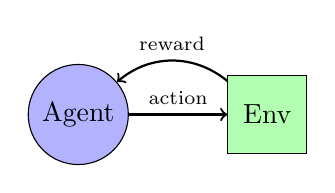
\begin{tikzpicture}[scale=0.6]
                    \node[draw, circle, fill=blue!30, minimum size=1cm] (a) at (0,0) {Agent};
                    \node[draw, rectangle, fill=green!30, minimum size=1cm] (e) at (4,0) {Env};
                    \draw[->, thick] (a) -- node[above] {\scriptsize action} (e);
                    \draw[->, thick] (e) to[bend right=40] node[above] {\scriptsize reward} (a);
                \end{tikzpicture}
            \end{center}
        \end{column}

        \begin{column}{0.48\textwidth}
            \textbf{Model-Based RL}
            \begin{itemize}
                \item Learn a model of the world
                \item Simulate outcomes internally
                \item More sample efficient
            \end{itemize}

            \vspace{0.3cm}
            \begin{center}
                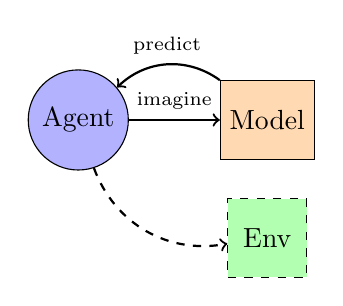
\begin{tikzpicture}[scale=0.6]
                    \node[draw, circle, fill=blue!30, minimum size=1cm] (a) at (0,0) {Agent};
                    \node[draw, rectangle, fill=orange!30, minimum size=1cm] (m) at (4,0) {Model};
                    \node[draw, rectangle, fill=green!30, dashed, minimum size=1cm] (e) at (4,-2.5) {Env};
                    \draw[->, thick] (a) -- node[above] {\scriptsize imagine} (m);
                    \draw[->, thick] (m) to[bend right=40] node[above] {\scriptsize predict} (a);
                    \draw[->, thick, dashed] (a) to[bend right=40] (e);
                \end{tikzpicture}
            \end{center}
        \end{column}
    \end{columns}
\end{frame}

%-----------------------------------------------
% SLIDE: Sample Efficiency
%-----------------------------------------------
\begin{frame}{Sample Efficiency}
    \begin{center}
        \textit{How many interactions does the agent need to learn?}
    \end{center}

    \vspace{0.5cm}
    \begin{columns}[T]
        \begin{column}{0.55\textwidth}
            \begin{center}
                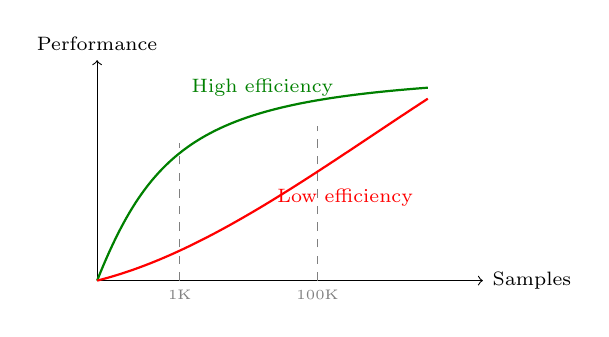
\begin{tikzpicture}[scale=0.7]
                    % Axes
                    \draw[->] (0,0) -- (7,0) node[right] {\scriptsize Samples};
                    \draw[->] (0,0) -- (0,4) node[above] {\scriptsize Performance};

                    % High sample efficiency (steep curve)
                    \draw[thick, green!50!black] (0,0) .. controls (1,2.5) and (2,3.2) .. (6,3.5);
                    \node[green!50!black] at (3,3.5) {\scriptsize High efficiency};

                    % Low sample efficiency (gradual curve)
                    \draw[thick, red] (0,0) .. controls (2,0.5) and (4,2) .. (6,3.3);
                    \node[red] at (4.5,1.5) {\scriptsize Low efficiency};

                    % Sample count markers
                    \draw[gray, dashed] (1.5,0) -- (1.5,2.5);
                    \node[below, gray] at (1.5,0) {\tiny 1K};
                    \draw[gray, dashed] (4,0) -- (4,2.8);
                    \node[below, gray] at (4,0) {\tiny 100K};
                \end{tikzpicture}
            \end{center}
        \end{column}

        \begin{column}{0.42\textwidth}
            \textbf{Why it matters:}
            \begin{itemize}
                \item Real-world interactions are expensive
                \item Time to train
                \item Compute resources
            \end{itemize}

            \vspace{0.3cm}
            \textbf{Improving efficiency:}
            \begin{itemize}
                \item Experience replay
                \item Better exploration
                \item Transfer learning
            \end{itemize}
        \end{column}
    \end{columns}

    \vspace{0.3cm}
    \begin{center}
        \fbox{Sample efficiency = performance gained per interaction}
    \end{center}
\end{frame}

\section{Implementation}
%-----------------------------------------------
% Section: Implementation
%-----------------------------------------------
\begin{frame}
    \begin{center}
        \vfill
        {\Huge \textbf{Implementation}} {\color{red}\textbf{TODO}}
        \vfill
    \end{center}
\end{frame}

\section{Conclusion}
%-----------------------------------------------
% Section: Conclusion
%-----------------------------------------------
\begin{frame}
    \begin{center}
        \vfill
        {\Huge \textbf{Conclusion}}
        \vfill
    \end{center}
\end{frame}

%-----------------------------------------------
% SLIDE: Applications
%-----------------------------------------------
\begin{frame}{Applications \hfill {\color{red}\textbf{TODO}}}
    \begin{columns}[T]
        \begin{column}{0.48\textwidth}
            \textbf{Games \& Simulation}
            \begin{itemize}
                \item AlphaGo, AlphaZero
                \item OpenAI Five (Dota 2)
                \item Atari games
            \end{itemize}

            \vspace{0.3cm}
            \textbf{Robotics}
            \begin{itemize}
                \item Manipulation tasks
                \item Locomotion
                \item Autonomous navigation
            \end{itemize}
        \end{column}

        \begin{column}{0.48\textwidth}
            \textbf{Real-World Systems}
            \begin{itemize}
                \item Autonomous vehicles
                \item Resource management
                \item Data center cooling
            \end{itemize}

            \vspace{0.3cm}
            \textbf{Other Domains}
            \begin{itemize}
                \item Recommendation systems
                \item Financial trading
                \item Healthcare optimization
            \end{itemize}
        \end{column}
    \end{columns}
\end{frame}

%-----------------------------------------------
% SLIDE: Limitations - Sample Inefficiency
%-----------------------------------------------
\begin{frame}{Limitations: Sample Inefficiency \hfill {\color{red}\textbf{TODO}}}
    \begin{itemize}
        \item \textbf{Humanoid locomotion}: 50--100 million frames to learn basic walking
        \item \textbf{Atari games}: 200 million frames (equivalent to 38 days of gameplay)
        \item \textbf{Real robots}: Hours/days of physical interaction
    \end{itemize}

    \vspace{0.5cm}
    \begin{center}
        \textit{``Deep RL is popular because it's the only area in ML where it's socially acceptable to train on the test set.''} -- Alex Irpan
    \end{center}

    \vspace{0.3cm}
    \begin{center}
        \fbox{Sample efficiency is the biggest bottleneck for real-world RL}
    \end{center}
\end{frame}

%-----------------------------------------------
% SLIDE: Limitations - Unreliability
%-----------------------------------------------
\begin{frame}{Limitations: Unreliability \hfill {\color{red}\textbf{TODO}}}
    \begin{itemize}
        \item \textbf{Sensitive to initial conditions}
        \begin{itemize}
            \item Same algorithm, same hyperparameters, different random seed
            \item Results can vary dramatically between runs
        \end{itemize}

        \item \textbf{Hyperparameter sensitivity}
        \begin{itemize}
            \item Small changes can break training completely
            \item Extensive tuning required for each new task
        \end{itemize}

        \item \textbf{Reproducibility challenges}
        \begin{itemize}
            \item Published results often hard to replicate
            \item ``Works on my machine'' problem
        \end{itemize}
    \end{itemize}

    \vspace{0.3cm}
    \begin{center}
        \fbox{RL algorithms often work sometimes, but not reliably}
    \end{center}
\end{frame}

%-----------------------------------------------
% SLIDE: Limitations (cont.)
%-----------------------------------------------
\begin{frame}{Limitations (cont.)}
    \begin{itemize}
        \item \textbf{Reward Engineering}
        \begin{itemize}
            \item Designing good reward functions is difficult
            \item Reward hacking and unintended behaviors
        \end{itemize}

        \item \textbf{Sim-to-Real Gap}
        \begin{itemize}
            \item Policies trained in simulation may not transfer
            \item Domain randomization helps but not perfect
        \end{itemize}

        \item \textbf{Safety \& Stability}
        \begin{itemize}
            \item Exploration can be dangerous
            \item Training instability in deep RL
        \end{itemize}
    \end{itemize}
\end{frame}

%-----------------------------------------------
% SLIDE: Future Methods - Bayesian RL
%-----------------------------------------------
\begin{frame}{Future Methods: Bayesian RL}
    \begin{center}
        \textit{What if the agent could reason about its own uncertainty?}
    \end{center}

    \vspace{0.5cm}
    \begin{columns}[T]
        \begin{column}{0.48\textwidth}
            \textbf{Standard RL:}
            \begin{itemize}
                \item Point estimates of Q-values
                \item Explore via $\epsilon$-greedy
                \item No uncertainty quantification
            \end{itemize}
        \end{column}

        \begin{column}{0.48\textwidth}
            \textbf{Bayesian RL:}
            \begin{itemize}
                \item Probability distributions over Q
                \item Explore where uncertain
                \item Principled exploration
            \end{itemize}
        \end{column}
    \end{columns}

    \vspace{0.5cm}
    \begin{center}
        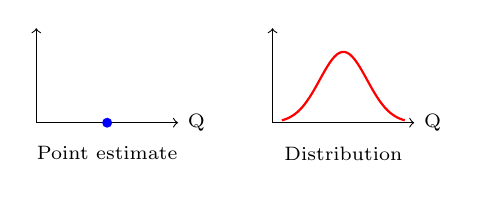
\begin{tikzpicture}[scale=0.6]
            % Point estimate
            \draw[->] (0,0) -- (3,0) node[right] {\scriptsize Q};
            \draw[->] (0,0) -- (0,2);
            \fill[blue] (1.5,0) circle (3pt);
            \node[below] at (1.5,-0.3) {\scriptsize Point estimate};

            % Distribution
            \draw[->] (5,0) -- (8,0) node[right] {\scriptsize Q};
            \draw[->] (5,0) -- (5,2);
            \draw[thick, red, domain=5.2:7.8, samples=50] plot (\x, {1.5*exp(-2*(\x-6.5)^2)});
            \node[below] at (6.5,-0.3) {\scriptsize Distribution};
        \end{tikzpicture}
    \end{center}

    \vspace{0.3cm}
    \begin{center}
        \fbox{Bayesian RL: maintain beliefs over value functions}
    \end{center}
\end{frame}

%-----------------------------------------------
% SLIDE: Future Methods - Distributional RL
%-----------------------------------------------
\begin{frame}{Future Methods: Distributional RL}
    \begin{center}
        \textit{What if we learned the full distribution of returns?}
    \end{center}

    \vspace{0.5cm}
    \begin{columns}[T]
        \begin{column}{0.48\textwidth}
            \textbf{Standard RL:}
            \begin{itemize}
                \item Learn expected return $\mathbb{E}[G]$
                \item Single value per state-action
                \item Ignores risk/variance
            \end{itemize}

            \vspace{0.3cm}
            \begin{center}
                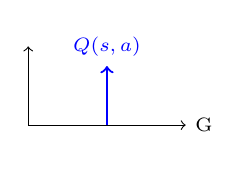
\begin{tikzpicture}[scale=0.5]
                    \draw[->] (0,0) -- (4,0) node[right] {\scriptsize G};
                    \draw[->] (0,0) -- (0,2);
                    \draw[thick, blue, ->] (2,0) -- (2,1.5);
                    \node[above, blue] at (2,1.5) {\scriptsize $Q(s,a)$};
                \end{tikzpicture}
            \end{center}
        \end{column}

        \begin{column}{0.48\textwidth}
            \textbf{Distributional RL:}
            \begin{itemize}
                \item Learn full distribution $Z(s,a)$
                \item Captures risk and variance
                \item Better feature learning
            \end{itemize}

            \vspace{0.3cm}
            \begin{center}
                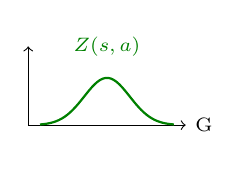
\begin{tikzpicture}[scale=0.5]
                    \draw[->] (0,0) -- (4,0) node[right] {\scriptsize G};
                    \draw[->] (0,0) -- (0,2);
                    \draw[thick, green!50!black, domain=0.3:3.7, samples=50] plot (\x, {1.2*exp(-1.5*(\x-2)^2)});
                    \node[above, green!50!black] at (2,1.5) {\scriptsize $Z(s,a)$};
                \end{tikzpicture}
            \end{center}
        \end{column}
    \end{columns}

    \vspace{0.3cm}
    \begin{center}
        \fbox{Distributional RL: $Q(s,a) = \mathbb{E}[Z(s,a)]$ but $Z$ carries more information}
    \end{center}
\end{frame}

%-----------------------------------------------
% SLIDE: Future Methods (cont.)
%-----------------------------------------------
\begin{frame}{Future Methods (cont.)}
    \begin{itemize}
        \item \textbf{Imitation Learning}
        \begin{itemize}
            \item Learn from expert demonstrations
            \item Bypasses reward engineering problem
        \end{itemize}

        \item \textbf{Model-Based RL}
        \begin{itemize}
            \item Learn a model of the environment
            \item Plan using the learned model (more sample efficient)
        \end{itemize}

        \item \textbf{Offline RL}
        \begin{itemize}
            \item Learn from logged data without exploration
            \item Safer deployment in critical applications
        \end{itemize}
    \end{itemize}
\end{frame}

%-----------------------------------------------
% SLIDE: Future Methods (cont. 2)
%-----------------------------------------------
\begin{frame}{Future Methods (cont.)}
    \begin{itemize}
        \item \textbf{Foundation Models for RL}
        \begin{itemize}
            \item Large pretrained models as world models
            \item Transfer learning across tasks
        \end{itemize}

        \item \textbf{Multi-Agent RL}
        \begin{itemize}
            \item Cooperative and competitive settings
            \item Emergent behaviors and communication
        \end{itemize}

        \item \textbf{Human-in-the-Loop RL}
        \begin{itemize}
            \item RLHF (Reinforcement Learning from Human Feedback)
            \item Aligning agents with human preferences
        \end{itemize}
    \end{itemize}
\end{frame}

%-----------------------------------------------
% SLIDE: References
%-----------------------------------------------
\begin{frame}{References}
    \begin{itemize}
        \item Sutton, R. S., \& Barto, A. G. (2018). \textit{Reinforcement Learning: An Introduction} (2nd ed.). MIT Press.
        \item OpenAI. \textit{Spinning Up in Deep RL}. \url{https://spinningup.openai.com/}
        \item Irpan, A. (2018). \textit{Deep Reinforcement Learning Doesn't Work Yet}. \url{https://www.alexirpan.com/2018/02/14/rl-hard.html}
    \end{itemize}
\end{frame}

\end{document}
